\PassOptionsToPackage{dvipsnames}{xcolor}
\documentclass[10pt, oneside]{article}   	% use "amsart" instead of "article" for AMSLaTeX format
\usepackage{geometry}                		% See geometry.pdf to learn the layout options. There are lots.
\geometry{letterpaper}                   		% ... or a4paper or a5paper or ... 
%\geometry{landscape}                		% Activate for rotated page geometry
%\usepackage[parfill]{parskip}    		% Activate to begin paragraphs with an empty line rather than an indent
\usepackage{graphicx}				% Use pdf, png, jpg, or eps§ with pdflatex; use eps in DVI mode
								% TeX will automatically convert eps --> pdf in pdflatex		
\usepackage{setspace}
\setstretch{0.5}


\usepackage{lmodern}
\usepackage{amsmath,amssymb,amsthm,enumitem,mathtools,xpatch}
\usepackage{bm}
\usepackage[most]{tcolorbox}
\usepackage[dvipsnames]{xcolor}
\newcommand*{\simsym}{\mathord\sim}\usepackage{amsthm}
\usepackage{float}
\usepackage{mathrsfs}
\usepackage{wrapfig, lipsum, amsthm, thmtools}
\usepackage{gensymb}
\usepackage{geometry}
 \geometry{
 a4paper,
 total={170mm,257mm},
 left=15mm,
 right = 15mm,
 top=15mm,
 bottom = 20mm
 }

\newcommand*{\Perm}[2]{{}^{#1}\!P_{#2}}%
\newcommand*{\Comb}[2]{{}^{#1}C_{#2}}%

\usepackage[framemethod=tikz]{mdframed}

\theoremstyle{definition}
\newtheorem*{exmp*}{Example}

\newtheorem*{defn*}{Definition}
\surroundwithmdframed[backgroundcolor=white]{defn*}

\newtheorem{cor*}{Corollary}
\surroundwithmdframed[backgroundcolor=white]{cor*}

\newtheorem*{prop*}{Proposition}
\surroundwithmdframed[backgroundcolor=white]{prop*}

\newtheorem*{thm*}{Theorem}
\surroundwithmdframed[backgroundcolor=white]{thm*}


% tikz for probability tree

\usepackage[latin1]{inputenc}
\usepackage{tikz}
\usetikzlibrary{trees,calc,angles,positioning,intersections}

% pgfplot
\usepackage{pgfplots}
\pgfplotsset{width=10cm,compat=1.9}

% pgfplotslibrary
\usepgfplotslibrary{fillbetween}

% quotations dirty talk
\usepackage{dirtytalk}

% floor ceiling
\DeclarePairedDelimiter\ceil{\lceil}{\rceil}
\DeclarePairedDelimiter\floor{\lfloor}{\rfloor}

% diag table
\usepackage{diagbox}

% math circle
\makeatletter
\newcommand\mathcircled[1]{%
  \mathpalette\@mathcircled{#1}%
}
\newcommand\@mathcircled[2]{%
  \tikz[baseline=(math.base)] \node[draw,circle,inner sep=1pt] (math) {$\m@th#1#2$};%
}
\makeatother


\title{Introductory Probability and Statistical Applications, Second Edition \\
\large{Paul L. Meyer}}
\author{Notes and Solutions by David A. Lee}
\date{}							% Activate to display a given date or no date

\begin{document}
\maketitle
\section*{Solutions to Chapter 7: Further Characteristics of Random Variables}

Unfinished Problems: 7.48

\begin{enumerate}[label=7.\arabic*]
\itemsep0em 
%Question 7.1
\item  \begin{tcolorbox}[
  colback=Cerulean!5!white,
  colframe=Cerulean!75!black]
\textbf{Find the expected value of the following random variables.}
\end{tcolorbox}

	\begin{enumerate}
	%Question 7.1(a)
	\item  \begin{tcolorbox}[
	  colback=Cerulean!5!white,
	  colframe=Cerulean!75!black]
	\textbf{The random variable $\bm{X}$ defined in Problem 4.1.}
	\end{tcolorbox}
	
	Problem 4.1 involves a coin such that when tossed, heads comes up three times as often as tails. The coin is tossed three times, and $X$ is the number of heads that appear. From the solutions set to chapter 4, we have $P(X = 0) = 1/64, P(X = 1) = 9/64, P(X = 2) = 27/64, P(X = 3) = 27/64$. Then we calculate:
	
	\[ E[X] = \sum^3_{x=0} xp(x) = 0 \cdot 1/64 + 1 \cdot 9/64 + 2 \cdot 27/64 + 3 \cdot 27/64 = \boxed{9/4} \]
	
	%Question 7.1(b)
	\item  \begin{tcolorbox}[
	  colback=Cerulean!5!white,
	  colframe=Cerulean!75!black]
	\textbf{The random variable $\bm{X}$ defined in Problem 4.2.}
	\end{tcolorbox}
	
	Problem 4.2 features a lot containing 25 items, 5 of which are defective, with 4 chosen at random, both with and without replacement. We let $X$ be the number of defectives found. From the solutions set to chapter 4, we have, in the case with replacement
	
	 \[ P(X=0) = 0.4096, P(X = 1) = 0.4096, P(X = 2) = 0.1536, P(X = 3) = 0.0256, P(X = 4) = 0.0016 \]
	 
	 and in the case without replacement:
	 
	  \[ P(X=0) = 0.3830, P(X = 1) = 0.4506, P(X = 2) = 0.1502, P(X = 3) = 0.0158, P(X = 4) = 0.0004 \]

	Then we need only calculate the expectation of $X$ in both cases.
	
	With replacement:
	
	\[ E[X] = \sum^4_{x=0} x p(x) = 1 \cdot 0.4096 + 2 \cdot 0.1536 + 3 \cdot 0.0256 + 4 \cdot 0.0016 = \boxed{0.8} \]
	
	Without replacement:
	
	\[ E[X] = \sum^4_{x=0} x p(x) = 1 \cdot 0.4506 + 2 \cdot 0.1502 + 3 \cdot 0.0158 + 4 \cdot 0.0004 = \boxed{0.8} \]
	
	%Question 7.1(c)
	\item  \begin{tcolorbox}[
	  colback=Cerulean!5!white,
	  colframe=Cerulean!75!black]
	\textbf{The random variable $\bm{T}$ defined in Problem 4.6.}
	\end{tcolorbox}
	
	Problem 4.6 describes the consecutive launching of rockets in 5 attempts, or until a successful launch is achieved. The probability of a successful launch is 0.8, and each attempt is independent from one another. Each initial launch costs $K$ dollars, with subsequent launches costing $K/3$ dollars, and a successful launch yields $C$ dollars in revenue. We let $T$ be the net cost of the experiment, and determine the expectation of $T$.
	
	As determined in the solution set for chapter 4, we have $P(T = C-K) = 0.8, P(T = C - 4K/3) = 0.16, P(T = C - 5K/3) = 0.032, P(T = C - 2K) = 0.0064, P(T = C - 7K/3) = 0.00128$. Then the expectation is given by:
	
	\begin{align*}
	E[T] &= (C-K) P(T = C-K) + (C - 4K/3) P(T = C - 4K/3) + (C - 5K/3) P(T = C - 5K/3) \\ 
	&\quad + (C - 2K) P(T = C - 2K) + (C - 7K/3) P(T = C - 7K/3) \\
	&= \boxed{0.99968 - 1.08245 K}
	\end{align*}
	
	%Question 7.1(d)
	\item  \begin{tcolorbox}[
	  colback=Cerulean!5!white,
	  colframe=Cerulean!75!black]
	\textbf{The random variable $\bm{X}$ defined in Problem 4.18.}
	\end{tcolorbox}
	
	Problem 4.18 describes the life length of an electronic device, represented by $X$, which has pdf $f(x) = k / x^n$ over $2000 \leq x \leq 10000$. In the general case,
	
	\[ k = \frac{(n-1) 2^{n-1} \cdot 10^{4(n-1)}}{10^{n-1} - 2^{n-1}} \]
	
	as derived in the solutions set for chapter 4. In the case of continuous variables, we calculate the expectation as follows:
	
	\begin{align*}
	E[X] = \int^{10000}_{2000} x f(x) dx &= \int^{10000}_{2000} kx^{-(n-1)} dx \\
	&= \boxed{ \frac{k}{n-2} (2000^{-(n-2)} - 10000^{-(n-2)})  }
	\end{align*}
	
	Upon inspection, it is apparent that this equation does not work in the case of $n = 2$. Here we can simply calculate
	
	\[ E[X] = \int^{10000}_{2000} kx^{-1} \ dx = 2500 \ln 5 \approx \boxed{4023.6} \]
	
	\end{enumerate}
	
%Question 7.2
\item  \begin{tcolorbox}[
  colback=Cerulean!5!white,
  colframe=Cerulean!75!black]
\textbf{Show that $\bm{E[X]}$ does not exist for the random variable $\bm{X}$ defined in Problem 4.25.}
\end{tcolorbox}

Problem 4.25 deals with the life length of a radio tube, denoted by $X$, with pdf $f(x) = 100/x^2, x > 100$. Then the expectation is calculated as

\[ E[X] = \lim_{b \rightarrow +\infty} \int^b_{100} x \Big( \frac{100}{x^2} \Big) dx =  \lim_{b \rightarrow + \infty} 100 (\ln b - \ln 100)\] 

Since the definite integral diverges, the expectation does not exist.

%Question 7.3
\item  \begin{tcolorbox}[
  colback=Cerulean!5!white,
  colframe=Cerulean!75!black]
\textbf{The following represents the probability distribution of $\bm{D}$, the daily demand of a certain product. Evaluate $\bm{E[D]}$.}

\begin{align*}
\bm{d:}& \ \bm{1, 2, 3, 4, 5,} \\
\bm{P(D = d):}& \ \bm{0.1, 0.1, 0.3, 0.3, 0.2}
\end{align*}
\end{tcolorbox}

\[ E[D] = \sum^5_{d=1} d P(D = d) = 1(0.1) + 2(0.1) + 3(0.3) + 4(0.3) + 5(0.2) = \boxed{3.4} \]

%Question 7.4
\item  \begin{tcolorbox}[
  colback=Cerulean!5!white,
  colframe=Cerulean!75!black]
\textbf{In the manufacture of petroleum, the distilling temperature, say $\bm{T}$ (degrees centigrade), is crucial in determining the quality of the final product. Suppose that $\bm{T}$ is considered as a random variable uniformly distributed over (150,300).}

\textbf{Suppose that it costs $\bm{C_1}$ dollars to produce one gallon of petroleum. If the oil distills at a temperature less than $\bm{200^\circ}$C, the product is known as naphtha and sells for $C_2$ dollars per gallon. If it is distilled at a temperature greater than $\bm{200^\circ}$C, it is known as refined oil distillate and sells for $\bm{C_3}$ dollars per gallon. Find the expected net profit (per gallon).}
\end{tcolorbox}

By uniform distribution, $f(T) = \frac{1}{150}$ on $150 \leq T \leq 300$. If naphtha is produced, then the net profit is given by $NP = C_2 - C_1$, and if refined oil distillate is produced, then the net profit is $NP = C_3 - C_1$. The probabilities of producing naphtha, and consequently of each respective net profit, is

\begin{align*}
P(T < 200) &= \int^{200}_{150} \frac{1}{150} \ dT = \frac{1}{3} = P(C_2 - C_1) \\
P(T \geq 200) &= \int^{300}_{200} \frac{1}{150} \ dT = \frac{2}{3} = P(C_3 - C_1) 
\end{align*}

Therefore, the expectation of the net profit per gallon is

\begin{align*}
E[NP] &= (C_2 - C_1) P(C_2 - C_1) + (C_3 - C_1) P(C_3 - C_1) \\
&= \boxed{\frac{C_2 + 2 C_3 - 3 C_1}{3}}
\end{align*}

%Question 7.5
\item  \begin{tcolorbox}[
  colback=Cerulean!5!white,
  colframe=Cerulean!75!black]
\textbf{A certain alloy is formed by combining the melted mixture of two metals. The resulting alloy contains a certain percent of lead, say $\bm{X}$, which may be considered as a random variable. Suppose that $\bm{X}$ has the following pdf:}

\[ \bm{f(x) = \frac{3}{5} 10^{-5} x (100-x), \qquad 0 \leq x \leq 100} \]

\textbf{Suppose that $\bm{P}$, the net profit realized in selling this alloy (per pound), is the following function of the percent content of lead: $\bm{P = C_1 + C_2 X}$. Compute the expected profit (per pound).}
\end{tcolorbox}

The insight to remember is the linear operator property of expectation, namely

\[ E[P] = C_1 + C_2 E[X] \]

where

\[ E[X] = \int^{100}_0 \frac{3}{5} 10^{-5} x^2 (100-x) \ dx = 50 \]

Therefore

\[E[P] = \boxed{C_1 + 50 C_2} \]

%Question 7.6
\item  \begin{tcolorbox}[
  colback=Cerulean!5!white,
  colframe=Cerulean!75!black]
\textbf{Suppose that an electronic device has a life length $\bm{X}$ (in units of 1000 hours) which is considered as a continuous random variable with the following pdf:}

\[ \bm{f(x) = e^{-x}, \qquad x > 0} \]

\textbf{Suppose that the cost of manufacturing one such item is \$2.00. The manufacturer sells the item for \$5.00, but guarantees a total refund if $\bm{X \leq 0.9}$. What is the manufacturer's expected profit per item?}
\end{tcolorbox}

Using the distribution, we have

\[ P(X \leq 0.9) = \int^{0.9}_0 e^{-x} \ dx = 1 - e^{-0.9} \]

Therefore, the probability that the item warrants a refund is $1 - e^{-0.9}$, and that it does not is $e^{-0.9}$. The expectation of the profit is thus

\[ E[\text{Profit}] = (5-2) e^{-0.9} + (-2) (1 - e^{-0.9}) = \boxed{\$ 0.03} \]

%Question 7.7
\item  \begin{tcolorbox}[
  colback=Cerulean!5!white,
  colframe=Cerulean!75!black]
\textbf{The first 5 repetitions of an experiment cost \$10 each. All subsequent repetitions cost \$5 each. Suppose that the experiment is repeated until the first successful outcome occurs. If the probability of a successful outcome always equals 0.9, and if the repetitions are independent, what is the expected cost of the entire operation?}
\end{tcolorbox}

Let $C_1$ be the cost from the first five attempts. Its expected value is

\[ E[C_1] = \sum^5_{n=1} 10n (0.1)^{n-1} (0.9) \]

Let $C_2$ be the cost for all future attempts. Its expected value is

\[ E[C_2] = \sum_{n=1}^\infty (50 + 5n) (0.1)^{5 + (n-1)} (0.9) \]

The expected cost of the total operation, then, is given by $E[C_1 + C_2]$. Evaluating analytically, one can use the fact that $\sum^m_{n=1} r^n = \frac{r - r^{m+1}}{1-r}$, and differentiate to find that $\sum^m_{n=1} nr^{n-1} = \frac{mr^{m+1} - (m+1) r^m + 1}{(1-r)^2}$. But it is simpler to evaluate numerically, for which we obtain $E[C_1 + C_2] = E[C_1] + E[C_2] = \boxed{\$ 11.11}$.

%Question 7.8
\item  \begin{tcolorbox}[
  colback=Cerulean!5!white,
  colframe=Cerulean!75!black]
\textbf{A lot is known to contain 2 defective and 8 nondefective items. If these items are inspected at random, one after another, what is the expected number of items that must be chosen \textit{for inspection} in order to remove all the defective ones?}
\end{tcolorbox}

Let $X$ be the number of items picked to clear the lot of defects. Consider the following possible outcomes:

$X = 2$
\begin{align*}
P(D, D) &= \Big( \frac{2}{10} \Big) \Big( \frac{1}{9} \Big) = 2/90 
\end{align*}

$X = 3$
\begin{align*}
P(N,D,D) &= \Big( \frac{8}{10} \Big) \Big( \frac{2}{9} \Big) \Big( \frac{1}{8} \Big) = 2/90 \\
P(D, N, D) &= \Big( \frac{2}{10} \Big) \Big( \frac{8}{9} \Big) \Big( \frac{1}{8} \Big) = 2/90 
\end{align*}

$X = 4$
\begin{align*}
P(N, N, D,D) &= \Big( \frac{8}{10} \Big) \Big( \frac{7}{9} \Big) \Big( \frac{2}{8} \Big) \Big( \frac{1}{7} \Big) = 2/90 \\
P(N, D, N,D) &= \Big( \frac{8}{10} \Big) \Big( \frac{2}{9} \Big) \Big( \frac{7}{8} \Big) \Big( \frac{1}{7} \Big) = 2/90 \\
P(D, N, N,D) &= \Big( \frac{2}{10} \Big) \Big( \frac{8}{9} \Big) \Big( \frac{7}{8} \Big) \Big( \frac{1}{7} \Big) = 2/90 \\
\end{align*}

Notice a pattern? Any particular outcome for any value of $X$ is $2/90$. We may generalize the probability that $X$ items must be chosen for inspection as

\[ P(X = n) = (n-1) \frac{2}{90} \]

The $n-1$ term represents that for whatever $X=n$, the last item must be defective by definition, for we say we inspected $X = n$ items when the $n$-th and final item we inspect turns out to be the second of the defective items. This then leaves $n-1$ unique ``outcomes" for the other defective item (namely, it can occupy the 1st, 2nd, ..., $n-1$-th position in the sequence of inspected items). Then the expected number of items that must be chosen for inspection for clearing the defective items is

\[ E[X] = \sum^{10}_{n=2} n(n-1) \frac{2}{90} = \boxed{ 7 \frac{1}{3} } \]

\textbf{Note:} Meyer lists $7 \frac{2}{15}$ as his answer. I disagree, unless an astute reader can identify if I have made an error. 

%Question 7.9
\item  \begin{tcolorbox}[
  colback=Cerulean!5!white,
  colframe=Cerulean!75!black]
\textbf{A lot of 10 electric motors must either be totally rejected or is sold, depending on the outcome of the following procedure: Two motors are chosen at random and inspected. If one or more are defective, the lot is rejected. Otherwise it is accepted. Suppose that each motor costs \$75 and is sold for \$100. If the lot contains 1 defective motor, what is the manufacturer's expected profit?}
\end{tcolorbox}

It follows from the premise that we may either choose one defective and one nondefective, or two nondefective motors. Since there is 1 defective and 9 nondefective motors, we may apply the hypergeometric probability and find

\begin{align*}
P(\text{Defective}) &= \frac{\binom{1}{1} \binom{9}{1}}{\binom{10}{2}} = 0.2 \\
P(\text{Non-defective}) &= \frac{\binom{1}{0} \binom{9}{2}}{\binom{10}{2}} = 0.8
\end{align*}

Since we have ten motors that each cost \$75, let $C = \$750$ be the total cost for the set of motors. If sold, the set will earn \$1,000, leading to a net profit of \$250. If the set cannot be sold, the net profit (loss) will be -\$750. Therefore the expectation of the net profit is given by

\[ E[\text{net profit}] = 250(0.8) + (-750)(0.2) = \boxed{\$50} \]

%Question 7.10
\item  \begin{tcolorbox}[
  colback=Cerulean!5!white,
  colframe=Cerulean!75!black]
\textbf{Suppose that $\bm{D}$, the daily demand for an item, is a random variable with the following probability distribution:}

\[ \bm{P(D=d) = C 2^d / d!,  \quad d = 1, 2, 3, 4} \]
\end{tcolorbox}

	\begin{enumerate}
	%Question 7.10(a)
	\item  \begin{tcolorbox}[
	  colback=Cerulean!5!white,
	  colframe=Cerulean!75!black]
	\textbf{Evaluate the constant $\bm{C}$.}
	\end{tcolorbox}
	
	By the Kolmogorov axioms for probability, we must have $C \Big[ \sum^4_{d=1} \frac{2^d}{d!} \Big] = 1$, which implies $\boxed{C = 1/6}$.
	
	%Question 7.10(b)
	\item  \begin{tcolorbox}[
	  colback=Cerulean!5!white,
	  colframe=Cerulean!75!black]
	\textbf{Compute the expected demand.}
	\end{tcolorbox}
	
	Calculating the corresponding probabilities for each of the values the daily demand can take on, the expectation is tabulated as
	
	\[ E[X] = \Big( 1 \cdot 2 + 2 \cdot 2 + 3 \cdot \frac{4}{3} + 4 \cdot \frac{2}{3} \Big) \frac{1}{6} = \boxed{\frac{19}{9}} \]
	
	%Question 7.10(c)
	\item  \begin{tcolorbox}[
	  colback=Cerulean!5!white,
	  colframe=Cerulean!75!black]
	\textbf{Suppose that an item is sold for \$5.00. A manufacturer produces $\bm{K}$ items daily. Any item which is not sold at the end of the day must be discarded at a loss of \$3.00. }
	\end{tcolorbox}
	
		\begin{enumerate}
		%Question 7.10(c)(i)
		\item  \begin{tcolorbox}[
	 	 colback=Cerulean!5!white,
	 	 colframe=Cerulean!75!black]
		\textbf{Find the probability distribution of the daily profit, as a function of $\bm{K}$.}
		\end{tcolorbox}
		
		Our profit equation is $5d - 3(K-d) (= 8d - 3K)$. The first term represents the proceeds from $d$ sales at \$5.00 per item, and the second is the total loss of $K-d$ unsold units at \$3.00 per item. To 		be pedantic, we can further mandate that $K \geq d$; namely, that the most demand can be met is by however many items $K$ the manufacturer produces.
		
		Therefore, the probability distributions for each value of $K$ are:
		
		\begin{center}
		\begin{tikzpicture}[scale=0.75]
	\begin{axis}
	[% 
	scatter/classes={%
		a={mark=square*,blue},%
		b={mark=triangle*,red},%
		c={mark=o,draw=black}},
		xlabel={$\text{Profit}$},
		ylabel={$P(\text{Profit})$},
		xtick={0},
		xticklabels={$5 (d= \text{1,2,3,4})$},x tick label style={rotate=45,anchor=east},
		ytick={0, 0.33, 0.67, 1},
		yticklabels={$0$,$1/3$, $2/3$, $1$},
		ymin=-0.1,ymax=1.1]
	\addplot[scatter,only marks,%
		scatter src=explicit symbolic]%
	table[meta=label] {
x     y      label
0      1   a       
	};
	\end{axis}
	\node[align=center,font=\bfseries, xshift=1.5em, yshift=1em] (title) 
    at (current bounding box.north)
    {$\bm{K=1}$};
\end{tikzpicture}
		\begin{tikzpicture}[scale=0.75]
	\begin{axis}
	[% 
	scatter/classes={%
		a={mark=square*,blue},%
		b={mark=triangle*,red},%
		c={mark=o,draw=black}},
		xlabel={$\text{Profit}$},
		ylabel={$P(\text{Profit})$},
		xtick={0, 1},
		xticklabels={$2 (d=1)$, $10 (d=\text{2,3,4})$},x tick label style={rotate=45,anchor=east},
		ytick={0, 0.33, 0.67, 1},
		yticklabels={$0$,$1/3$, $2/3$, $1$},
		ymin=-0.1,ymax=1.1]
	\addplot[scatter,only marks,%
		scatter src=explicit symbolic]%
	table[meta=label] {
x     y      label
0      0.33   a     
1      0.67   a        
	};
	\end{axis}
	\node[align=center,font=\bfseries, xshift=1.5em, yshift=1em] (title) 
    at (current bounding box.north)
    {$\bm{K=2}$};
\end{tikzpicture}
\end{center}

\begin{center}
	\begin{tikzpicture}[scale=0.75]
	\begin{axis}
	[% 
	scatter/classes={%
		a={mark=square*,blue},%
		b={mark=triangle*,red},%
		c={mark=o,draw=black}},
		xlabel={$\text{Profit}$},
		ylabel={$P(\text{Profit})$},
		xtick={0, 1, 2},
		xticklabels={$-1 (d=1)$, $7 (d=2)$, $15 (d = \text{3,4})$},x tick label style={rotate=45,anchor=east},
		ytick={0, 0.33, 0.67, 1},
		yticklabels={$0$,$1/3$, $2/3$, $1$},
		ymin=-0.1,ymax=1.1]
	\addplot[scatter,only marks,%
		scatter src=explicit symbolic]%
	table[meta=label] {
x     y      label
0      0.33   a     
1      0.33   a     
2      0.33   a  
	};
	\end{axis}
	\node[align=center,font=\bfseries, xshift=1.5em, yshift=1em] (title) 
    at (current bounding box.north)
    {$\bm{K=3}$};
\end{tikzpicture}
\begin{tikzpicture}[scale=0.75]
	\begin{axis}
	[% 
	scatter/classes={%
		a={mark=square*,blue},%
		b={mark=triangle*,red},%
		c={mark=o,draw=black}},
		xlabel={$\text{Profit}$},
		ylabel={$P(\text{Profit})$},
		xtick={0, 1, 2, 3},
		xticklabels={$-8 (d=1)$, $4 (d=2)$, $12 (d = 3)$, $20 (d = 4)$},x tick label style={rotate=45,anchor=east},
		ytick={0, 0.33, 0.67, 1},
		yticklabels={$0$,$1/3$, $2/3$, $1$},
		ymin=-0.1,ymax=1.1]
	\addplot[scatter,only marks,%
		scatter src=explicit symbolic]%
	table[meta=label] {
x     y      label
0      0.33   a     
1      0.33   a     
2      0.22   a
3      0.11   a     
	};
	\end{axis}
	\node[align=center,font=\bfseries, xshift=1.5em, yshift=1em] (title) 
    at (current bounding box.north)
    {$\bm{K=4}$};
\end{tikzpicture}
\end{center}
		
		%Question 7.10(c)(ii)
		\item  \begin{tcolorbox}[
	 	 colback=Cerulean!5!white,
	 	 colframe=Cerulean!75!black]
		\textbf{How many items should be manufactured to maximize the expected daily profit?}
		\end{tcolorbox}
		
		The conditional expectations for each value of $K$ are
		
		\begin{align*}
		E[\text{Profit} | K = 1] &= 5 \cdot 1 = 5 \\
		E[\text{Profit} | K = 2] &= 2 \cdot \frac{1}{3} + 10 \cdot \frac{2}{3} = \frac{22}{3} \\
		E[\text{Profit} | K = 3] &= \Big( -1 \cdot \frac{1}{3} \Big) + \Big( 7 \cdot \frac{1}{3} \Big) + \Big( 15 \cdot \frac{1}{3} \Big) = 7 \\
		E[\text{Profit} | K = 4] &= \Big( -8 \cdot \frac{1}{3} \Big) + \Big( 4 \cdot \frac{1}{3} \Big) + \Big( 12 \cdot \frac{2}{9} \Big) + \Big( 20 \cdot \frac{1}{9} \Big) = \frac{32}{9}
		\end{align*}
		
		Therefore, the maximum expected daily profit is attained for $\boxed{K = 2}$.
		
		\end{enumerate}
	
	\end{enumerate}

%Question 7.11
\item  \begin{tcolorbox}[
  colback=Cerulean!5!white,
  colframe=Cerulean!75!black]
  \textbf{[Intentionally blank]}
\end{tcolorbox}

	\begin{enumerate}
	%Question 7.11(a)
	\item  \begin{tcolorbox}[
	  colback=Cerulean!5!white,
	  colframe=Cerulean!75!black]
	\textbf{With $\bm{N = 50, p = 0.3}$, perform some computations to find that value of $\bm{k}$ which minimizes $\bm{E[X]}$ in Example 7.12.}
	\end{tcolorbox}
	
	Meyer Example 7.12 describes an algorithm for testing, in the most efficient manner, $N$ individuals for a characteristic taking on a positive or negative result. Either the $N$ persons may be tested individually using $N$ tests, or groups of $k$ specimens be tested such that $kn = N$ (i.e., there are $n$ such groups of $k$ individuals), meaning the number of tests needed will range from $n = N/k$ to $(k + 1)n = N + n$. In the former case, each of the $n$ groups could all test negative, implying each of their constituent individuals is negative; in the former, all of the $n$ groups test positive, and thus each of the $k$ constituents per group must be individually tested.
	
	The expected number of tests derived as a function of $N$ and $k$ is
	
	\[ E[X] = N [1 - (1-p)^k + k^{-1}] \]
	
	And for givens $N = 50, p = 0.3$, we graph the expectation as
	
		\begin{center}
	\begin{tikzpicture}[scale=0.75]
	\begin{axis}[
		scatter/classes={%
		a={mark=*,black},%
		b={mark=triangle*,red},%
		c={mark=o,draw=black}},
    		axis lines = left,
		ymax=75,
		ymin=45,
   		 xlabel = \( k \),
   		 ylabel = {\( E[X] \)},
		 xtick={0,1,2,3,4,10},
    		 xticklabels={$0$,$1$,$2$,$3$,$4$,$10$},
		 ytick={45,49.517,65,75},
		 yticklabels={$45$,$49.517$,$65$,$75$},
		]
	\addplot[domain=0:11, samples = 500, color=red, style=very thick]{50*(1 - (1 - 0.3)^x + 1/x)};
	\addplot[domain=0:30, samples = 500, color=blue, style=very thick] coordinates {(1, 65) (1, 0)};
	\addplot[domain=0:30, samples = 500, color=black, style=dotted] coordinates {(0, 65) (1, 65)};
	\addplot[domain=0:30, samples = 500, color=blue, style=very thick] coordinates {(2, 50.5) (2, 0)};
	\addplot[domain=0:30, samples = 500, color=black, style=dotted] coordinates {(0, 50.5) (2, 50.5)};
	\addplot[domain=0:30, samples = 500, color=blue, style=very thick] coordinates {(3, 49.517) (3, 0)};
	\addplot[domain=0:30, samples = 500, color=black, style=dotted] coordinates {(0, 49.517) (3, 49.517)};
	\addplot[domain=0:30, samples = 500, color=blue, style=very thick] coordinates {(4, 50.495) (4, 0)};
	\addplot[domain=0:30, samples = 500, color=black, style=dotted] coordinates {(0, 50.495) (4, 50.495)};
	
	\addplot[scatter,only marks,%
		scatter src=explicit symbolic]%
	table[meta=label] {
x     y      label     
1      65   a     
2      50.5   a
3      49.517   a     
4	50.495   a
	};
	\end{axis}
	\end{tikzpicture}
	\end{center}
	
	It is clear to see that $\lim_{k \rightarrow \infty} 50 [1 - (0.7)^k + k^{-1}] = 50$. Since $k$ can only take on integer values, it follows that the expectation is minimized at $\boxed{k=3}$ specimens per group, for an expected value of around $\boxed{50}$ tests.
	
	%Question 7.11(b)
	\item  \begin{tcolorbox}[
	  colback=Cerulean!5!white,
	  colframe=Cerulean!75!black]
	\textbf{Using the above values of $\bm{N}$ and $\bm{p}$ and using $\bm{k = 5, 10, 25}$, determine for each of these values of $\bm{k}$ whether ``group testing" is preferable.}
	\end{tcolorbox}
	
	The reader may verify that the aforementioned values of $k$ lead to expectations of 51.6, 53.6, and 52, respectively. Therefore, all are inferior to individual testing (requiring 50 tests).
	\end{enumerate}

%Question 7.12
\item  \begin{tcolorbox}[
  colback=Cerulean!5!white,
  colframe=Cerulean!75!black]
  \textbf{Suppose that $\bm{X}$ and $\bm{Y}$ are independent random variables with the following pdf's:}
  
  \[ \bm{f(x) = 8/x^3, x > 2; \quad g(y) = 2y, 0 < y < 1} \]
\end{tcolorbox}

	\begin{enumerate}
	%Question 7.12(a)
	\item  \begin{tcolorbox}[
	  colback=Cerulean!5!white,
	  colframe=Cerulean!75!black]
	\textbf{Find the pdf of $\bm{Z = XY}$.}
	\end{tcolorbox}
	
	We observe that $0 < z < +\infty$. Using the Mellin transform for the product of random variables, we let $u = x$ and $z = xy$. Then $y = z/u$, and $0 < y < 1  \implies 0 < z/u < 1 \implies z < u < + \infty$. Then we write
	
	\[ P(Z) = \int^{+\infty}_{z} f(u) g \Big( \frac{z}{u} \Big) \Big| \frac{1}{u} \Big| \ du = \int^{+\infty}_{z} \frac{8}{u^3} \Big( \frac{2z}{u} \Big) \frac{1}{u} \ du = \boxed{ \frac{4}{z^3}, \quad 2 < z < +\infty} \]
	
	Next, we suppose that $u = y$ and $z = xu$. Then $x = z/u$, and $2 < x \implies 2 < z/u \implies 2u < z \implies 0 < u < z/2 \implies 0 < z < 2$. Thus we write
	
	\[ P(Z) = \int^{z/u}_0 2u \Big( \frac{8u^3}{z^3} \Big) \frac{1}{u} \ du = \boxed{\frac{z}{4}, \quad 0 < z < 2} \]
	
	The reader may verify that the Kolmogorov axioms are satisfied.
	
	%Question 7.12(b)
	\item  \begin{tcolorbox}[
	  colback=Cerulean!5!white,
	  colframe=Cerulean!75!black]
	\textbf{Obtain $\bm{E[Z]}$ in two ways:}
	\end{tcolorbox}
	
		\begin{enumerate}
		%Question 7.12(b)(i)
		\item  \begin{tcolorbox}[
		  colback=Cerulean!5!white,
		  colframe=Cerulean!75!black]
		\textbf{using the pdf of $\bm{Z}$ as obtained in (a).}
		\end{tcolorbox}
		
		By premise, independence of $X,Y$ implies $f(x,y) = g(x) h(y)$. Then by LOTUS,
		
		\[ E[Z] = \int^{+\infty}_2 \int^1_0 (xy) \Big( \frac{8}{x^3} \Big) (2y) \ dy dx = \boxed{\frac{8}{3}} \]
		
		%Question 7.12(b)(ii)
		\item  \begin{tcolorbox}[
		  colback=Cerulean!5!white,
		  colframe=Cerulean!75!black]
		\textbf{Directly, without using the pdf of $\bm{Z}$.}
		\end{tcolorbox}
		
		Using $P(Z)$, we calculate
		
		\[ E[Z] = \int^2_0 z \Big( \frac{z}{4} \Big) \ dz + \int^{+\infty}_2 z \Big( \frac{4}{z^3} \Big) \ dz = \boxed{\frac{8}{3}} \]
		
		\end{enumerate}
	\end{enumerate}

%Question 7.13
\item  \begin{tcolorbox}[
  colback=Cerulean!5!white,
  colframe=Cerulean!75!black]
  \textbf{Suppose that $\bm{X}$ has pdf}
  
  \[ \bm{ f(x) = 8/x^3, \quad x > 2} \]
  
  \textbf{Let $\bm{W = \frac{1}{3}X}$.}
\end{tcolorbox}

	\begin{enumerate}
	%Question 7.13(a)
	\item  \begin{tcolorbox}[
	  colback=Cerulean!5!white,
	  colframe=Cerulean!75!black]
	\textbf{Evaluate $\bm{E[W]}$ using the pdf of $\bm{W}$.}
	\end{tcolorbox}

	For functions of one random variable, $g(w) = f(x) | \frac{dx}{dw} |$. Then $g(w) = \frac{8}{(3w)^3} \cdot 3 = \frac{8}{9w^3}, \quad \frac{2}{3} < w < +\infty$. Then $E[W] = \int^{+\infty}_{2/3} \big( \frac{8}{9w^3} \big) w \ dw = \boxed{4/3}$.
	
	%Question 7.13(b)
	\item  \begin{tcolorbox}[
	  colback=Cerulean!5!white,
	  colframe=Cerulean!75!black]
	\textbf{Evaluate $\bm{E[W]}$ without using the pdf of $\bm{W}$.}
	\end{tcolorbox}
	
	By LOTUS, $E[W] = \int^{+\infty}_2 \big( \frac{1}{3}x \big) \big( \frac{8}{x^3} \big) \ dx = \boxed{4/3}$.
	\end{enumerate}

%Question 7.14
\item  \begin{tcolorbox}[
  colback=Cerulean!5!white,
  colframe=Cerulean!75!black]
  \textbf{A fair die is tossed 72 times. Given that $\bm{X}$ is the number of times six appears, evaluate $\bm{E[X^2]}$.}
  \end{tcolorbox}
  
In the discrete form of LOTUS, $E[Y] = E[H(X)] = \sum^\infty_{j=1} H(x_j) P(x_j)$. The probability that six appears exactly $n$ times in 72 rolls is $P(X = n) = \binom{72}{n} \big( \frac{1}{6} \big)^n \big( \frac{5}{6} \big)^{72-n} $. By LOTUS, $E[X^2] = \sum^{72}_{n=1} n^2 \binom{72}{n} \big( \frac{1}{6} \big)^n \big( \frac{5}{6} \big)^{72-n}  = \boxed{154}$.

%Question 7.15
\item  \begin{tcolorbox}[
  colback=Cerulean!5!white,
  colframe=Cerulean!75!black]
  \textbf{Find the expected value and variance of the random variables $\bm{Y}$ and $\bm{Z}$ of Problem 5.2.}
  \end{tcolorbox}
  
  Here, $X$ has pdf $f(x) = 1/2, 1 \leq X \leq 3$. Then $E[X] = \int^3_1 \frac{x}{2} \ dx = 2, E[X^2] = \int^3_1 \frac{x^2}{2} \ dx = 13/3 $, and $V[X] = E[X^2] -  E[X]^2 = 1/3$.
  
	\begin{enumerate}
	%Question 7.15(a)
	\item  \begin{tcolorbox}[
	  colback=Cerulean!5!white,
	  colframe=Cerulean!75!black]
	\textbf{$\bm{Y = 3X + 4}$}
	\end{tcolorbox}
	
	Applying the properties of expectation and variance, $E[Y] = 3 E[X] + 4 = \boxed{10}$ and $V[Y] = V[3X + 4] = 9 V[X] = \boxed{3}$.
	
	%Question 7.15(b)
	\item  \begin{tcolorbox}[
	  colback=Cerulean!5!white,
	  colframe=Cerulean!75!black]
	\textbf{$\bm{Z = e^X}$}
	\end{tcolorbox}
	
	By LOTUS, $E[Z] = \int^3_1 \frac{e^x}{2} \ dx = \boxed{\frac{e^3 - e}{2}}$ and $E[Z^2] = \int^3_1 \frac{e^{2x}}{2} \ dx = \frac{e^6 - e^2}{4}$. Then $V[Z] = E[Z^2] - E[Z]^2 = \boxed{\frac{e^4 - e^2}{2}}$.
	\end{enumerate}

%Question 7.16
\item  \begin{tcolorbox}[
  colback=Cerulean!5!white,
  colframe=Cerulean!75!black]
  \textbf{Find the expected value and variance of the random variable $\bm{Y}$ of Problem 5.3.}
  \end{tcolorbox}
  
  Here, $X$ has pdf $f(x) = e^{-x}, x > 0$, and $Y = X^3$. By LOTUS, $E[Y] = \int^{+\infty}_0 x^3 e^{-x} \ dx = \boxed{6}$. Moreover, $E[Y^2] = \int^{+\infty}_0 x^6 e^{-x} \ dx = 720$. Then $V[Y] = E[Y^2] - E[Y]^2 = \boxed{684}$.
  
%Question 7.17
\item  \begin{tcolorbox}[
  colback=Cerulean!5!white,
  colframe=Cerulean!75!black]
  \textbf{Find the expected value and variance of the random variables $\bm{Y}$ and $\bm{Z}$ of Problem 5.5.}
  \end{tcolorbox}
  
  Here, $X$ is uniformly distributed over $(0,1)$. Thus $f(x) = 1, 0 \leq X \leq 1$, and $E[X] = \int^1_0 x \ dx = 1/2$ and $E[X^2] = \int^1_0 x^2 \ dx = 1/3$.
  
  	\begin{enumerate}
	%Question 7.17(a)
	\item  \begin{tcolorbox}[
	  colback=Cerulean!5!white,
	  colframe=Cerulean!75!black]
	\textbf{$\bm{Y = X^2 + 1}$}
	\end{tcolorbox}
	
	We have $E[Y] = E[X^2 + 1] = E[X^2] + 1 = \boxed{4/3}$. Then $Y^2 = (X^2 + 1)^2 = X^4 + 2X^2 + 1$, meaning $E[Y^2] = E[X^4] + 2 E[X^2] + 1 = 28/15$. Lastly, $V[Y] = E[Y^2] = E[Y]^2 = \boxed{4/45}$.
	
	%Question 7.17(b)
	\item  \begin{tcolorbox}[
	  colback=Cerulean!5!white,
	  colframe=Cerulean!75!black]
	\textbf{$\bm{Z = 1/(X + 1)}$}
	\end{tcolorbox}	
	
	We have $E[Z] = \int^1_0 \frac{1}{x + 1} \ dx = \boxed{\ln 2}$ and $E[Z^2] = \int^1_0 \frac{1}{(x + 1)^2} \ dx = 1/2$. Then $V[Z] = E[Z^2] - E[Z]^2 = \boxed{1/2 - [\ln(2)]^2}$
	\end{enumerate}
	
%Question 7.18
\item  \begin{tcolorbox}[
  colback=Cerulean!5!white,
  colframe=Cerulean!75!black]
  \textbf{Find the expected value and variance of the random variables $\bm{Y, Z,}$ and $\bm{W}$ of Problem 5.6.}
  \end{tcolorbox}
  
  Here, $X$ is uniformly distributed over $(-1,1)$, so $f(x) = 1/2, -1 \leq X \leq 1$.
  
  	\begin{enumerate}
	%Question 7.18(a)
	\item  \begin{tcolorbox}[
	  colback=Cerulean!5!white,
	  colframe=Cerulean!75!black]
	\textbf{$\bm{Y = \sin (\pi / 2) X}$}
	\end{tcolorbox}
	
	By LOTUS, $E[Y] = \int^1_{-1} \sin (\pi/2) x \ dx = \boxed{0}$. Furthermore, $E[Y^2] = \int^1_{-1} \frac{1}{2} \sin^2 (\pi / 2) x \ dx$, which, using the identity $\sin^2 x = \frac{1 - \cos 2x}{2}$, can be evaluated as $1/2$. Then $V[Y] = E[Y^2] - E[Y]^2 = \boxed{1/2}$.
	
	%Question 7.18(b)
	\item  \begin{tcolorbox}[
	  colback=Cerulean!5!white,
	  colframe=Cerulean!75!black]
	\textbf{$\bm{Z = \cos (\pi / 2) X}$}
	\end{tcolorbox}
	
	By LOTUS, $E[Z] = \int^1_{-1} \frac{1}{2} \cos (\pi/2) x \ dx = \boxed{2 / \pi}$. Moreover, $E[Z^2] = \int^1_{-1} \frac{1}{2} \cos^2 (\pi/2) x \ dx$, which, using the identity $\cos^2 x = \frac{1 + \cos 2x}{2}$, can be evaluated as $1/2$. Then $V[Z] = E[Z^2] - E[Z]^2 = \boxed{\frac{1}{2\pi^2} (\pi^2 - 8)}$.
	
	%Question 7.18(c)
	\item  \begin{tcolorbox}[
	  colback=Cerulean!5!white,
	  colframe=Cerulean!75!black]
	\textbf{$\bm{W = |X|}$}
	\end{tcolorbox}
	
	Here,
	
	\begin{align*}
	W &= \begin{dcases}
	 x, \quad 0 \leq x \leq 1 \\
	 -x, \quad -1 \leq x \leq 0
	 \end{dcases}
	 \end{align*}
	 
	 By LOTUS, $E[W] = \int^1_0 \frac{x}{2} \ dx - \int^0_{-1} \frac{x}{2} \ dx = \boxed{1/2}$, and $E[W^2] = \int^1_{-1} \frac{x^2}{2} \ dx = 1/3$. Then $V[W] = E[W^2] - E[W]^2 = \boxed{1/12}$.
	
	\end{enumerate}
	
%Question 7.19
\item  \begin{tcolorbox}[
  colback=Cerulean!5!white,
  colframe=Cerulean!75!black]
  \textbf{Find the expected value and variance of the random variables $\bm{V}$ and $\bm{S}$ of Problem 5.7.}
  \end{tcolorbox}
  
Here, we have the radius of a sphere represented as a continuous random variable $R$ with pdf $f(r) = 6r(1-r), 0 < r < 1$, and are asked to find the expectation and variance of the volume $V$ and surface area $S$ of the sphere.

\textbf{Volume}

The volume of a sphere is $V = \frac{4}{3} \pi r^3$. By LOTUS, evaluating $E[V] = \int^1_0 \frac{4}{3} \pi r^3 (6r(1-r)) \ dr$ and $E[V^2] = \int^1_0 \frac{16}{9} \pi^2 r^6 (6r(1-r)) \ dr$ yields $\boxed{4\pi / 15}$ and $\boxed{4 \pi^2 / 27}$, respectively. It then follows that $V[V] = E[V^2] - E[V]^2 = \boxed{52 \pi^2 / 675}$.

\textbf{Surface Area}

The surface area of a sphere is $S = 4 \pi r^2$. By LOTUS, $E[S] = \int^1_0 4 \pi r^2 (6r(1-r)) \ dr = \boxed{6 \pi / 5}$ and $E[S^2] = \int^1_0 16 \pi^2 r^4 (6r(1-r)) \ dr = 16 \pi^2 / 7$. It follows that $V[S] = E[S^2] - E[S]^2 = \boxed{148 \pi^2 / 175}$.

%Question 7.20
\item  \begin{tcolorbox}[
  colback=Cerulean!5!white,
  colframe=Cerulean!75!black]
  \textbf{Find the expected value and variance of the random variable $\bm{Y}$ of Problem 5.10 for each of the three cases.}
  \end{tcolorbox}
  
  	\begin{center}
	\begin{tikzpicture}[scale=0.75]
	\begin{axis}[
    		axis lines = center,
		xmax=5,
		xmin=-5,
		ymax=4,
		ymin=0,
   		 xlabel = \( X \),
   		 ylabel = {\( Y \)},
		 xtick={-3,-1,1,3},
    		 xticklabels={$-x_0$,$-a$,$a$,$x_0$},
		 ytick={},
		 yticklabels={},
		]
	\addplot[samples=500,domain=3:5, color=black]{2};
	\addplot[samples=500,domain=-5:-3, color=black]{2};
	\addplot[samples=500,domain=-3:-1, color=black]{-x-1};
	\addplot[samples=500,domain=1:3, color=black]{x-1};
	\end{axis}
	\end{tikzpicture}
	\end{center}
	
	\begin{enumerate}
	%Question 7.20(a)
	\item  \begin{tcolorbox}[
	  colback=Cerulean!5!white,
	  colframe=Cerulean!75!black]
	\textbf{$\bm{k < a}$}
	\end{tcolorbox}
	
	Since $Y = 0$ for all $X \in (-a, a)$, $\boxed{E[Y] = 0, V[Y] = 0}$.
	
	%Question 7.20(b)
	\item  \begin{tcolorbox}[
	  colback=Cerulean!5!white,
	  colframe=Cerulean!75!black]
	\textbf{$\bm{a < k < x_0}$}
	\end{tcolorbox}
	
	The piecewise definition of $Y$ is
	
	\[ Y = \begin{dcases}
	-\frac{y_0}{x_0 - a} X - \frac{ay_0}{x_0 - a}, & -k < x < -a \\
	0, &-a \leq x \leq a \\
	\frac{y_0}{x_0 - a} X - \frac{ay_0}{x_0 - a}, &a < x < k
	\end{dcases} \]
	
	Using LOTUS, we will calculate the expectation for each segment of $Y$, and then sum together.
	
	$\bm{ -k < x < -a }$
	
	\begin{align*}
	E[Y] &= \int^{-a}_{-k} \Big[ -\frac{y_0}{x_0-a} x - \frac{ay_0}{x_0-a} \Big] \frac{1}{2k} \ dx \\
	&= \frac{1}{2k} \Big[ -\frac{y_0}{x_0 - a} \frac{a^2-k^2}{2} - \frac{ay_0}{x_0 - a} (k-a) \Big]
	\end{align*}
	
	$\bm{-a \leq x \leq a}$
	
	\begin{align*}
	E[Y] = 0
	\end{align*}
	
	$\bm{a < x < k}$
	
	\begin{align*}
	E[Y] &= \int^k_a \Big[ \frac{y_0}{x_0 - a} x - \frac{ay_0}{x_0 - a} \Big] \frac{1}{2k} \ dx \\
	&= \frac{1}{2k} \Big[ \frac{y_0}{x_0 - a} \frac{k^2 - a^2}{2} - \frac{ay_0}{x_0 - a} (k - a) \Big]
	\end{align*}
	
	Summing the constituent expectations yields $\boxed{E[Y] = \frac{y_0 (k-a)^2}{2k (x_0 - a)}}$.
	
	In the alternative, using the pdf of $Y$ previously derived in 5.10
	
	\[ g(y) = \begin{dcases}
	\frac{a}{k}, & y = 0 \\
	\frac{x_0 - a}{k y_0}, & 0 < y < \frac{y_0 (k-a)}{x_0 - a}
	\end{dcases} \]
	
	We may calculate the expectation of $Y$ from its definition as follows (since $y=0$ in the first segment, we may ignore it to calculate $E[Y]$)
	
	\begin{align*}
	E[Y] &= \int^{\frac{y_0 (k-a)}{x_0 - a}}_0 \Big( \frac{x_0 - a}{k y_0} \Big) y \ dy \\
	&= \boxed{\frac{y_0 (k-a)^2}{2k (x_0 - a)}}
	\end{align*}
	
	Next, we derive the variance of $Y$ by way of the definition $V[Y] = E[Y^2] - E[Y]^2$. We have $Y^2$ defined as
	
	\[ Y^2 = \begin{dcases}
	\frac{y^2_0}{(x_0 - a)^2} X^2 + \frac{2a y^2_0}{(x_0 - a)^2} X + \frac{a^2 y^2_0}{(x_0 - a)^2}, & -k < x < -a \\
	0, &-a \leq x \leq a \\
	\frac{y^2_0}{(x_0 - a)^2} X^2 - \frac{2ay^2_0}{(x_0 - a)^2} X + \frac{a^2 y^2_0}{(x_0 - a)^2}, &a < x < k
	\end{dcases} \]
	
	Deriving the $E[Y^2]$ for each of the branches yields
	
	$\bm{ -k < x < -a }$
	
	\begin{align*}
	E[Y^2] &= \frac{1}{2k} \int^{-a}_{-k} \Big[ \frac{y^2_0}{(x_0 - a)^2} X^2 + \frac{2a y^2_0}{(x_0 - a)^2} X + \frac{a^2 y^2_0}{(x_0 - a)^2} \Big] \ dx \\
	&= \frac{y^2_0}{6k} \frac{(k-a)^3}{(x_0 - a)^2}
	\end{align*}
	
	$\bm{-a \leq x \leq a}$
	
	\begin{align*}
	E[Y^2] = 0
	\end{align*}
	
	$\bm{a < x < k}$
	
	\begin{align*}
	E[Y^2] &= \frac{1}{2k} \int^k_a \Big[ \frac{y^2_0}{(x_0 - a)^2} X^2 - \frac{2ay^2_0}{(x_0 - a)^2} X + \frac{a^2 y^2_0}{(x_0 - a)^2} \Big] \ dx \\
	&= \boxed{ \frac{y^2_0}{6k} \frac{(k-a)^3}{(x_0 - a)^2} }
	\end{align*}
	
	Combining the constituent expectations, we get $\boxed{E[Y^2] = \frac{y^2_0}{3k} \frac{(k -a)^3}{(x_0 - a)^2} }$. \\
	Therefore, $\boxed{V[Y] = \frac{y^2_0}{3k} \frac{(k-a)^3}{(x_0 - a)^2} - \Big[ \frac{y_0 (k-a)^2}{2k (x_0 - a)} \Big]^2 }$.
	
	Equivalently, we may use $g(y)$ to find
	
	\begin{align*}
	E[Y^2] &= \int^{\frac{y_0 (k-a)}{x_0 - a}}_0 \Big( \frac{x_0 - a}{k y_0} \Big) y^2 \ dy \\
	&= \boxed{\frac{y^2_0 (k-a)^3}{3k (x_0 - a)^2}}
	\end{align*}

	Which then leads us to the aforementioned result for $V[Y]$.
	
	%Question 7.20(c)
	\item  \begin{tcolorbox}[
	  colback=Cerulean!5!white,
	  colframe=Cerulean!75!black]
	\textbf{$\bm{k > x_0}$}
	\end{tcolorbox}
	
	In this case, we previously derived $g(y)$ as
	
	\[ g(y) = \begin{dcases}
	a/k, & y=0 \\
	\frac{x_0 - a}{k y_0}, &0 < y < y_0 \\
	1 - \frac{x_0}{k}, & y = y_0
	\end{dcases} \]
	
	Applying the definition of expectation, we get
	
	\begin{align*}
	E[Y] &= \int^{y_0}_0 \frac{x_0 - a}{ky_0} y \ dy + y_0 \Big( 1 - \frac{x_0}{k} \Big) \\
	&= \boxed{y_0 \Big[ 1 - \Big( \frac{x_0 + a}{2k} \Big) \Big]} \\
	E[Y^2] &= \int^{y_0}_0 \Big( \frac{x_0 - a}{k y_0} \Big) y^2 \ dy + y^2_0 \Big( 1 - \frac{x_0}{k} \Big) \\
	&= y^2_0 \Big[ 1 - \Big( \frac{2x_0 + a}{3k} \Big) \Big] \\
	V[Y] &= E[Y^2] - E[Y]^2 \\
	&= y^2_0 \Big[ 1 - \Big( \frac{2x_0 + a}{3k} \Big) \Big] - y^2_0 \Big[ 1 - \Big( \frac{x_0 + a}{2k} \Big) \Big]^2 \\
	&= \boxed{y^2_0 \Big[ \Big( \frac{x_0 + 2a}{3k} \Big) - \Big( \frac{x_0 + a}{2k} \Big)^2 \Big]}
	\end{align*}
	
	\end{enumerate}
	
	\textbf{Note:} My solution completely differs from Meyer's. Moreover, there are certain values for the parameters that give us negative variances for Meyer's solution, so I am confident mine are correct and the author's are not.
	
%Question 7.21
\item  \begin{tcolorbox}[
  colback=Cerulean!5!white,
  colframe=Cerulean!75!black]
  \textbf{Find the expected value and variance of the random variable $\bm{A}$ of Problem 6.7.}
  \end{tcolorbox}
  
  Since $X, Y$ are independent, $E(A) = E(XY) = E(X)E(Y)$. Then
  
  \[ E[A] = E[XY] = \int^2_1 x(x-1) \ dx \int^4_2 \frac{y}{2} \ dy + \int^3_2 x(-x + 3) \ dx \int^4_2 \frac{y}{2} \ dy = \boxed{6} \]
  
  We can verify this by calculating $\int_A a p(a) \ da$ for each of the constituent sections of the piecewise-defined $p(a)$, as derived in Problem 6.7. I leave this as an exercise to the reader.
  
  To calculate the variance, we will prove the following proposition.
  
  \begin{prop*}
  If $(X,Y)$ is a two-dimensional random variable with joint pdf $f(x,y)$ and $X, Y$ are independent random variables with pdf's $g(x), h(y)$, then $E[(XY)^2] = E[X^2 Y^2] = E[X^2] E[Y^2]$.
  \end{prop*}
  
  \begin{proof}
  
  By LOTUS for two-dimensional random variables,
  
  \begin{align*}
  E[(XY)^2] = E[X^2 Y^2] &= \int^{+\infty}_{-\infty} \int^{+\infty}_{-\infty} x^2 y^2 f(x,y) \ dx \ dy \\
  &= \int^{+\infty}_{-\infty} \int^{+\infty}_{-\infty} x^2 y^2 g(x) h(y) \ dx \ dy \\
  &= \int^{+\infty}_{-\infty} x^2 g(x) \ dx \int^{+\infty}_{-\infty} y^2 h(y) \ dy = E[X^2] E[Y^2]
  \end{align*}
  
  Now we can proceed with
  
  \begin{align*}
  E[A^2] &= E[X^2 Y^2] = \Bigg[ \int^2_1 x^2 (x-1) \ dx + \int^3_2 x^2 (-x + 3) \ dx \Bigg] \int^4_2 \frac{y^2}{2} \ dy = \frac{350}{9} \\
  V[A] &= E[A^2] - E[A]^2 = \boxed{\frac{26}{9}} 
  \end{align*}
  
  In the alternative, knowing that we may also define variance as $V[X] = E[(X - E[X])^2] = \int^{+\infty}_{-\infty} (x - E[X])^2 f(x) \ dx$, we can calculate $\int_A (a-6)^2 p(a) \ da$ across the constituent segments of $p(a)$ to find $\boxed{26/9}$.
  
  \end{proof}
  
%Question 7.22
\item  \begin{tcolorbox}[
  colback=Cerulean!5!white,
  colframe=Cerulean!75!black]
  \textbf{Find the expected value and variance of the random variable $\bm{H}$ of Problem 6.11.}
  \end{tcolorbox}
  
  By independence of $I, X$, we can write
  
  \begin{align*}
  E \Big[ \frac{2I}{X} \Big] &= 2 \int^5_3 \frac{1}{x} f(x) \ dx \int^{20}_{10} i g(i) \ di \\
  &= 2 \int^5_3 \frac{1}{2x} \ dx \int^{20}_{10} \frac{i}{10} \ di = \boxed{15 \ln \Big( \frac{5}{3} \Big)}
  \end{align*}
  
  In the alternative, using the pdf for $H$ derived in 6.11
  
  \[ q(h) =
\begin{dcases}
 \frac{1600-9h^2}{80h^2}, \quad 8 < h < 40/3  \\
 \frac{5h^2 - 80}{16 h^2}, \quad 4 < h < 20/3 
\end{dcases}
\]

We may also find $E[H] = \int_H h q(h) \ dh = \boxed{15 \ln \Big( \frac{5}{3} \Big)}$. To calculate $E[H^2]$, we write

\begin{align*}
E[4I^2 / X^2] &= 4 \int^5_3 \frac{1}{x^2} f(x) \ dx \int^{20}_{10} i^2 g(i) \ di \\
&= 4 \int^5_3 \frac{1}{2x^2} \ dx \int^{20}_{10} \frac{i^2}{10} \ di = 560/9
\end{align*}

Allowing us to conclude $V[H] = E[H^2] - E[H]^2 \approx \boxed{3.51}$. Similarly, $V[H] = \int_H (h - E[H])^2 q(h) \ dh \approx \boxed{3.51}$.
  
%Question 7.23
\item  \begin{tcolorbox}[
  colback=Cerulean!5!white,
  colframe=Cerulean!75!black]
  \textbf{Find the expected value and variance of the random variable $\bm{W}$ of Problem 6.13.}
  \end{tcolorbox}
  
  Calculating $E[W]$ and $E[W^2]$,
  
  \begin{align*}
  E[W] = E[I^2 R] &= \int^1_0 i^2 f(i) \ di \int^1_0 r g(r) \ dr \\
  &= \int^1_0 i^2 (6i(1-i)) \ di \int^1_0 2r^2 \ dr = \boxed{1/5} \\
  E[W^2] = E[I^4 R^2] &= \int^1_0 i^4 f(i) \ di \int^1_0 r^2 g(r) \ dr \\
  &= \int^1_0 i^2 (6i(1-i)) \ di \int^1_0 2r^3 \ dr = 1/14
  \end{align*}
  
  Therefore, $V[W] = E[W^2] - E[W]^2 = \boxed{11/350}$. In the alternative, $E[W] = \int^1_0 w p(w) \ dw = \boxed{1/5}$ and $V[W] = \int^1_0 (w - E[W])^2 p(w) \ dw = \boxed{11/350}$.

%Question 7.24
\item  \begin{tcolorbox}[
  colback=Cerulean!5!white,
  colframe=Cerulean!75!black]
  \textbf{Suppose that $\bm{X}$ is a random variable for which $\bm{E[X] = 10}$ and $\bm{V[X] = 25}$. For what positive values of $\bm{a}$ and $\bm{b}$ does $\bm{Y = aX - b}$ have expectation 0 and variance 1?}
  \end{tcolorbox}
  
  We wish to find $a, b$ such that $E[Y] = aE[X] - b = 0$ and $V[Y] = a^2 V[X] = 1$. From this we can derive $10a = b$ and $25a^2 = 1$, implying $\boxed{a = 1/5, b = 2}$.
  
  %Question 7.25
\item  \begin{tcolorbox}[
  colback=Cerulean!5!white,
  colframe=Cerulean!75!black]
  \textbf{Suppose that $\bm{S}$, a random voltage, varies between 0 and 1 volt and is uniformly distributed over that interval. Suppose that the signal $\bm{S}$ is perturbed by an additive, independent random noise $\bm{N}$ which is uniformly distributed between 0 and 2 volts.}
  \end{tcolorbox}
  
  	\begin{enumerate}
	  %Question 7.25(a)
	\item  \begin{tcolorbox}[
	  colback=Cerulean!5!white,
	  colframe=Cerulean!75!black]
	  \textbf{Find the expected voltage of the signal, taking noise into account.}
	  \end{tcolorbox}
	  
	  Since the voltages of the signal and noise are additive, the expectation of the total voltage $S+N$ is given by
	  
	  \[ E[S+N] = E[S] + E[N] = \int^1_0 s \ ds + \int^2_0 \frac{n}{2} \ dn = \boxed{3/2} \]
	  
	  %Question 7.25(b)
	\item  \begin{tcolorbox}[
	  colback=Cerulean!5!white,
	  colframe=Cerulean!75!black]
	  \textbf{Find the expected power when the perturbed signal is applied to a resistor of 2 ohms.}
	  \end{tcolorbox}
	  
	  Power is given by $P = V^2 / R$. For $V = S+N, R = 2$, we need only calculate
	  
	  \begin{align*}
	  E[P] &= \frac{1}{2} E[V^2] = \frac{1}{2} E[(S+N)^2] \\
	  &= \frac{1}{2} ( E[S^2] + 2E[SN] + E[N^2] ) \\
	  &= \frac{1}{2} \Big( \int^1_0 s^2 \ ds + 2 \int^1_0 s \ ds \int^2_0 \frac{n}{2} \ dn + \int^2_0 \frac{n^2}{2} \ dn \Big) = \boxed{4/3}
	  \end{align*}
	\end{enumerate}

%Question 7.26
\item  \begin{tcolorbox}[
  colback=Cerulean!5!white,
  colframe=Cerulean!75!black]
  \textbf{Suppose that $\bm{X}$ is uniformly distributed over $\bm{[-a, 3a]}$. Find the variance of $\bm{X}$.}
  \end{tcolorbox}
  
  By premise, $X$ has pdf $f(x) = \frac{1}{4a}$ over $-a \leq x \leq 3a$. We can calculate
  
  \begin{align*}
  E[X] &= \int^{3a}_{-a} \frac{x}{4a} \ dx = a \\
  E[X^2] &= \int^{3a}_{-a} \frac{x^2}{4a}\ dx = \frac{7}{3} a^2
  \end{align*}
  
  Therefore, $V[X] = E[X^2] - E[X]^2 = \boxed{4a^2 / 3}$.
  
%Question 7.27
\item  \begin{tcolorbox}[
  colback=Cerulean!5!white,
  colframe=Cerulean!75!black]
  \textbf{A target is made of three concentric circles of radii $\bm{1/ \sqrt{3}}, \bm{1},$ and $\bm{\sqrt{3}}$ feet. Shots within the inner circle count 4 points, within the next ring 3 points, and within the third ring 2 points. Shots outside the target count zero. Let $\bm{R}$ be the random variable representing the distance of the hit from the center. Suppose that the pdf of $\bm{R}$ is $\bm{f(r) = 2 / \pi (1+r^2), r > 0}$. Compute the expected value of the score after 5 shots.}
  \end{tcolorbox}
  
  The respective probabilities for each of the points are given by
  
  \begin{align*}
  P(\text{4 pts}) = P\Bigg( 0 \leq r \leq \frac{1}{\sqrt{3}} \Bigg) &= \int^{1/\sqrt{3}}_0 \frac{2}{\pi} \frac{1}{(1+r^2)} \ dr = \boxed{1/3} \\
  P(\text{3 pts}) = P\Bigg( \frac{1}{\sqrt{3}} < r \leq 1 \Bigg) &= \int^{1}_{1/\sqrt{3}} \frac{2}{\pi} \frac{1}{(1+r^2)} \ dr = \boxed{1/6} \\
  P(\text{2 pts}) = P( 1 < r \leq \sqrt{3} ) &= \int^{\sqrt{3}}_{1} \frac{2}{\pi} \frac{1}{(1+r^2)} \ dr = \boxed{1/6} \\
  P(\text{0 pts}) = P( \sqrt{3} < r ) &= \int^{+\infty}_{\sqrt{3}} \frac{2}{\pi} \frac{1}{(1+r^2)} \ dr = \boxed{1/3} 
  \end{align*}
  
  Making use of the fact that $\int \frac{1}{(1+x)^2} \ dx = \tan^{-1} x + C$. Now, we must invoke the notion that the expectation's additive property, namely that the expectation of a sum of random variables is the sum of the expectations of the constituent variables. Let $X_i$ be the number of points won on the $i$-th shot. Then let $Y$ be the total number of points won after 5 shots, or $Y = \sum^5_{i=1} X_i$. Since the distribution of outcomes for each $X_i$ are identical to one another, we have $E[X_i] = E[X_j]$ for each $i, j = 1,...,5$. For any $i$, $E[X_i] = 4(1/3)+3(1/6)+2(1/6) = 13/6$. Then $E[Y] = 5 \cdot 13/6 = \boxed{65/6}$.
  
%Question 7.28
\item  \begin{tcolorbox}[
  colback=Cerulean!5!white,
  colframe=Cerulean!75!black]
  \textbf{Suppose that the continuous random variable $\bm{X}$ has pdf}
  
  \[ \bm{f(x) = 2xe^{-x^2}, \quad x \geq 0} \]
  
  \textbf{Let $\bm{Y = X^2}$. Evaluate $\bm{E[Y]}$:}
  \end{tcolorbox}
  
	\begin{enumerate}
	%Question 7.28(a)
	\item  \begin{tcolorbox}[
	  colback=Cerulean!5!white,
	  colframe=Cerulean!75!black]
	  \textbf{directly without first obtaining the pdf of $\bm{Y}$,}
	  \end{tcolorbox}
	  
	  By LOTUS, we have
	  
	  \[ E[Y] = E[X^2] = \int^{+\infty}_0 2x^3 e^{-x^2} \ dx = \boxed{1} \] 
	  
	  Which can be evaluated using $u$-substitution twice or by a Gaussian integral table. 
	  
	  %Question 7.28(b)
	\item  \begin{tcolorbox}[
	  colback=Cerulean!5!white,
	  colframe=Cerulean!75!black]
	  \textbf{by first obtaining the pdf of $\bm{Y}$.}
	  \end{tcolorbox}
	  
	  By Meyer Theorem 5.2, the pdf of a random variable of the form $Y = X^2$ may be expressed as $g(y) = \frac{1}{2 \sqrt{y}} [f(\sqrt{y}) + f(-\sqrt{y})]$. Here, we have $g(y) = \frac{1}{2 \sqrt{y}} f(\sqrt{y}) = e^{-y}, y \geq 0$. Then we calculate
	  
	  \[ E[Y] = \int^{+\infty}_0 ye^{-y} \ dy = \boxed{1} \]
	\end{enumerate}

%Question 7.29
\item  \begin{tcolorbox}[
  colback=Cerulean!5!white,
  colframe=Cerulean!75!black]
  \textbf{Suppose that the two-dimensional random variable $\bm{(X,Y)}$ is uniformly distributed over the triangle in Fig. 7.15. Evaluate $\bm{V[X]}$ and $\bm{V[Y]}$.}
  \end{tcolorbox}
  
  	\begin{center}
	\begin{tikzpicture}[scale=0.75]
	\begin{axis}[
    		axis lines = center,
		y=1cm, % scaling y-axis
		x=5cm, % scaling x-axis
		xmax=1.5,
		xmin=-1.5,
		ymax=4,
		ymin=0,
   		 xlabel = \( x \),
   		 ylabel = {\( y \)},
		 xtick={-1,0,1},
    		 xticklabels={$-1$,$0$,$1$},
		 ytick={0},
		 yticklabels={$0$},
		]
		 \node (some node) at (50,300) (a) {}; % establishing reference nodes for placing labels below
		  \node (some node) at (250,300) (c) {};
	\addplot[samples=500,domain=0:1, color=black, style=thick]{3*x} node[above=1pt of c] {$(1,3)$}; % see syntax for placing labels relative to reference node
	\addplot[samples=500,domain=-1:0, color=black, style=thick]{-3*x} node[above=1pt of a] {$(-1,3)$};
	\addplot[thick, samples=50, smooth,domain=-1:1,black] coordinates {(-1,3)(1,3)};
	\addplot [only marks] table {
};
	\end{axis}
	\end{tikzpicture}
	\end{center}

Since $(X,Y)$ is uniformly distributed over the given triangle, its joint pdf is $f(x,y) = 1 / \text{area} = 1/3$. To derive the marginal pdf's of $X$ and $Y$, we calculate

\begin{align*}
g(x) &= \int^3_{-3x} \frac{1}{3} \ dy = 1 + x, \quad -1 \leq x \leq 0 \\
g(x) &= \int^3_{3x} \frac{1}{3} \ dy = 1 - x, \quad 0 < x \leq 1 \\
h(y) &= \int^{y/3}_{-y/3} \frac{1}{3} \ dx = \frac{2y}{9}, \quad 0 \leq y \leq 3
\end{align*}

Therefore, our pdf's are

\begin{align*}
g(x) &=
\begin{dcases}
1 + x, & -1 \leq x \leq 0 \\
1 - x, & 0 < x \leq 1 \\
\end{dcases} \\
h(y) &= \frac{2y}{9}, \quad 0 \leq y \leq 3
\end{align*}

Using the fact that $V[X] = \int (x-E[X])^2 f(x) \ dx$, we can calculate

\begin{align*}
E[X] &= \int^0_{-1} x(1+x) \ dx + \int^1_0 x(1-x) \ dx = 0 \\
V[X] &= \int^0_{-1} x^2 (1+x) \ dx + \int^1_0 x^2 (1-x) \ dx = \boxed{1/6} \\
E[Y] &= \int^3_0 \frac{2y^2}{9} \ dy = 2 \\
V[Y] &= \int^3_0 (y-2)^2 \frac{2y}{9} \ dy = \boxed{1/2}
\end{align*}

%Question 7.30
\item  \begin{tcolorbox}[
  colback=Cerulean!5!white,
  colframe=Cerulean!75!black]
  \textbf{Suppose that $\bm{(X,Y)}$ is uniformly distributed over the triangle in Fig. 7.16.}
  \end{tcolorbox}
  
    	\begin{center}
	\begin{tikzpicture}[scale=0.75]
	\begin{axis}[
    		axis lines = left,
		xmax=2.5,
		xmin=0,
		ymax=4.5,
		ymin=0,
   		 xlabel = \( x \),
   		 ylabel = {\( y \)},
		 xtick={0},
    		 xticklabels={$0$},
		 ytick={0},
		 yticklabels={$0$},
		]
		 \node (some node) at (195,25) (a) {}; % establishing reference nodes for placing labels below
		  \node (some node) at (200,385) (c) {};
	\addplot[samples=500,domain=0:2, color=black, style=thick]{2*x} node[above=1pt of c] {$(2,4)$}; % see syntax for placing labels relative to reference node
	\addplot[thick, samples=50, smooth,domain=-1:1,black] coordinates {(2,0)(2,4)} node[right=1pt of a] {$(2,0)$};
	\addplot [only marks] table {
};
	\end{axis}
	\end{tikzpicture}
	\end{center}
  
	\begin{enumerate}
	%Question 7.30(a)
	\item  \begin{tcolorbox}[
	  colback=Cerulean!5!white,
	  colframe=Cerulean!75!black]
	  \textbf{Obtain the marginal pdf of $\bm{X}$ and of $\bm{Y}$.}
	  \end{tcolorbox}
	  
	  As in the previous problem, given $(X,Y)$ uniformly distributed over the triangle, its joint pdf is $f(x,y) = 1 / \text{area} = 1/4$. The marginal pdf's are
	  
	  \begin{align*}
	  g(x) &= \int^{2x}_0 \frac{1}{4} \ dy = \boxed{x/2, \quad 0 \leq x \leq 2} \\
	  h(y) &= \int^2_{y/2} \frac{1}{4} \ dx = \boxed{ \frac{4 - y}{8}, \quad 0 \leq y \leq 4 }
	  \end{align*}
	  
	  \newpage
	  %Question 7.30(b)
	\item  \begin{tcolorbox}[
	  colback=Cerulean!5!white,
	  colframe=Cerulean!75!black]
	  \textbf{Evaluate $\bm{V[X]}$ and $\bm{V[Y]}$.}
	  \end{tcolorbox}
	  
	  We calculate
	  
	  \begin{align*}
	  E[X] &= \int^2_0 \frac{x^2}{2} \ dx = 4/3 \\
	  V[X] &= \int^2_0 (x - 4/3)^2 \frac{x}{2} \ dx = \boxed{2/9} \\
	  E[Y] &= \int^4_0 y \Big( \frac{4-y}{8} \Big) \ dy = 4/3 \\
	  V[Y] &= \int^4_0 (y - 4/3)^2 \Big( \frac{4-y}{8} \Big) \ dy = \boxed{4/9}
	  \end{align*}
	\end{enumerate}

%Question 7.31
\item  \begin{tcolorbox}[
  colback=Cerulean!5!white,
  colframe=Cerulean!75!black]
  \textbf{Suppose that $\bm{X}$ and $\bm{Y}$ are random variables for which $\bm{E[X] = \mu_x}$, $\bm{E[Y] = \mu_y}$, $\bm{V[X] = \sigma^2_x}$, and $\bm{V[Y] = \sigma^2_y}$. Using Theorem 7.7, obtain an approximation for $\bm{E[Z]}$ and $\bm{V[Z]}$, where $\bm{Z = X/Y}$.}
  \end{tcolorbox}
  
  By Meyer Theorem 7.7, if $Z = H(X,Y)$, and assuming independence of $X,Y$, then
  
  \begin{align*}
  E[Z] &\approx H(\mu_x, \mu_y) + \frac{1}{2} \Big[ \frac{\partial^2 H}{\partial x^2} \sigma^2_x + \frac{\partial^2 H}{\partial y^2} \sigma^2_y \Big] \\
  V[Z] &\approx \Big[ \frac{\partial H}{\partial x} \Big]^2 \sigma^2_x + \Big[ \frac{\partial H}{\partial y} \Big]^2 \sigma^2_y
  \end{align*}
  
  with partial derivatives evaluated at $(\mu_x, \mu_y)$. For $Z = H(X,Y) = X/Y$, we calculate $\partial H / \partial x = 1/y, \partial^2 H / \partial x^2 = 0, \partial H / \partial y = -x / y^2, \partial^2 H / \partial y^2 = 2x / y^3$. Then $E[Z] \approx \frac{\mu_x}{\mu_y} + \frac{1}{2} \Big[ \frac{2x}{y^3} \sigma^2_y \Big]$, and evaluated at $(\mu_x, \mu_y)$ we get
  
  \[ \boxed{ E[Z] \approx \frac{\mu_x}{\mu_y} + \frac{\mu_x}{\mu^3_y} \sigma^2_y } \]
  
  Moreover, $V[Z] \approx \Big( \frac{1}{y} \Big)^2 \sigma^2_x + \Big( -\frac{x}{y^2} \Big)^2 \sigma^2_y$, or at $(\mu_x, \mu_y)$
  
  \[ \boxed{V[Z] = \frac{1}{\mu^2_y} \sigma^2_x + \frac{\mu^2_x}{\mu^4_y} \sigma^2_y } \]

%Question 7.32
\item  \begin{tcolorbox}[
  colback=Cerulean!5!white,
  colframe=Cerulean!75!black]
  \textbf{Suppose that $\bm{X}$ and $\bm{Y}$ are independent random variables, each uniformly distributed over $\bm{(1,2)}$. Let $\bm{Z = X/Y}$.}
  \end{tcolorbox}
  
  	\begin{enumerate}
	%Question 7.32(a)
	\item  \begin{tcolorbox}[
	  colback=Cerulean!5!white,
	  colframe=Cerulean!75!black]
	  \textbf{Using Theorem 7.7, obtain approximate expressions for $\bm{E[Z]}$ and $\bm{V[Z]}$.}
	  \end{tcolorbox}
	  
	  We calculate $E[X] = E[Y] = \int^2_1 x \ dx = 3/2$ and $V[X] = V[Y] = \int^2_1 (x - 3/2)^2 \ dx = 1/12$. Inputting to the expressions derived in the aforementioned problem, we get approximations $\boxed{E[Z] \approx 28/27}$ and $\boxed{V[Z] \approx 2/27}$.
	  
	  %Question 7.32(b)
	\item  \begin{tcolorbox}[
	  colback=Cerulean!5!white,
	  colframe=Cerulean!75!black]
	  \textbf{Using Theorem 6.5, obtain the pdf of $\bm{Z}$ and then find the exact value of $\bm{E[Z]}$ and $\bm{V[Z]}$. Compare with (a).}
	  \end{tcolorbox}
	  
	  Using the Mellin transform for a quotient of random variables, let $z = x/y$ and $v = y$. Then $zy = x$, and by premise, it follows that $1 \leq zy \leq 2$. From this, we derive bounds $1/z \leq y \leq 2$ and $1 \leq y \leq 2/z$. Thus we piecewise integrate to find $g(z)$:
	  
	  \[ g(z) =
	  \begin{dcases}
	  \int^2_{1/z} v \ dv = 2 - \frac{1}{2z^2}, \quad \frac{1}{2} \leq z \leq 1 \\
	  \int^{2/z}_1 v \ dv = \frac{2}{z^2} - \frac{1}{2}, \quad 1 \leq z \leq 2
	  \end{dcases}
	  \]
	  
	  Therefore, the exact value of $E[Z]$ is given by
	  
	  \[ E[Z] = \int^1_{1/2} z \Big( 2 - \frac{1}{2z^2} \Big) \ dz + \int^2_1 z \Big( \frac{2}{z^2} - \frac{1}{2} \Big) \ dz \approx \boxed{1.0397} \]
	  
	  And $V[Z]$ by
	  
	  \[ V[Z] = \int^1_{1/2} (z - E[Z])^2 \Big( 2 - \frac{1}{2z^2} \Big) \ dz + \int^2_1 (z - E[Z])^2 \Big( \frac{2}{z^2} - \frac{1}{2} \Big) \ dz \approx \boxed{0.0856} \]
	  
	\end{enumerate}

%Question 7.33
\item  \begin{tcolorbox}[
  colback=Cerulean!5!white,
  colframe=Cerulean!75!black]
  \textbf{Show that if $\bm{X}$ is a continuous random variable with pdf $\bm{f}$ having the property that the graph of $\bm{f}$ is symmetric about $\bm{x = a}$, then $\bm{E[X] = a}$, provided that $\bm{E[X]}$ exists.}
  \end{tcolorbox}
  
  \begin{proof}
  By premise, the distribution of outcomes of $X$ is symmetric about $b$. Intuitively, we can see that if we subtract $b$ from $X$, we are ``recentering" the distribution about zero; simply put, the distribution of $X-b$ is now symmetric about the origin. Exploiting this fact, we can see that a reflection of the distribution $X-b$ about the vertical axis -- represented as the random variable $b - X$ -- is exactly the same distribution as initially. And two distributions that are identical must necessarily have the same characteristics, including its expectation. Therefore we can write $E[X - b] = E[b - X]$, implying $\boxed{E[X] = b}$.
  \end{proof}
  
%Question 7.34
\item  \begin{tcolorbox}[
  colback=Cerulean!5!white,
  colframe=Cerulean!75!black]
  \textbf{[Intentionally blank]}
  \end{tcolorbox}
  
  	\begin{enumerate}
	%Question 7.34(a)
	\item  \begin{tcolorbox}[
	  colback=Cerulean!5!white,
	  colframe=Cerulean!75!black]
	  \textbf{Suppose that the random variable $\bm{X}$ assumes the values -1 and 1 each with probability $\bm{\frac{1}{2}}$. Consider $\bm{P[|X - E[X]| \geq k \sqrt{V[X]}]}$ as a function of $\bm{k}$, $\bm{k > 0}$. Plot this function of $\bm{k}$ and, on the same coordinate system, plot the upper bound of the above probability as given by Chebyshev's inequality.} 
	  \end{tcolorbox}
	  
	  We have $E[X] = -1 (1/2) + 1 (1/2) = 0$, $E[X^2] = (-1)^2 (1/2) + (1)^2 (1/2) = 1$, and $V[X] = E[X^2] - E[X]^2 = 1$. Then our Chebyshev bound is given by $\boxed{P[|X| \geq k] \leq 1/k^2}$. In words, all this is saying is that the probability of $|X|$ being greater than $k$ standard deviations from the mean is less than or equal to $1 / k^2$ (put differently, $1/k^2$ is an upper bound).
	  
	  \begin{center}
	  \begin{tikzpicture}[scale=0.75]
	\begin{axis}
	[% 
	scatter/classes={%
		a={mark=square*,blue},%
		b={mark=triangle*,red},%
		c={mark=o,draw=black}},
		xlabel={$k$},
		ylabel={$P$},
		xtick={0, 1, 2, 3},
		xticklabels={$0$, $1$, $2$, $3$},
		ytick={0, 0.11, 0.25, 0.5, 1},
		yticklabels={$0$,$1/9$, $1/4$, $1/2$, $1$},
		ymin=0,ymax=1.1]
	\addplot[scatter,only marks,%
		scatter src=explicit symbolic]%
	table[meta=label] {
x     y      label
1      1   a     
1      1   b     
2      0.25   a
2      0   b     
3	0.11   a
3	0	b
	};
	\legend{$\text{Chebyshev bound}$,$P[|X| \geq k]$}
	\end{axis}
\end{tikzpicture}
\end{center}
	  
	  %Question 7.34(b)
	\item  \begin{tcolorbox}[
	  colback=Cerulean!5!white,
	  colframe=Cerulean!75!black]
	  \textbf{Same as (a) except that $\bm{P(X = -1) = \frac{1}{3}, P(X = 1) = \frac{2}{3}}$.} 
	  \end{tcolorbox}
	  
	  Here, $E[X] = -1 (1/3) + 1 (2/3) = 1/3, E[X^2] = (-1)^2 (1/3) + (1)^2 (2/3) = 1$, and $V[X] = E[X^2] - E[X]^2 = 8/9$. Then $\sigma = \sqrt{8}/3$, meaning our Chebyshev bound is $\boxed{P[|X - 1/3| \geq k \sqrt{8}/3] \leq 1/k^2}$. Graphically,
	  
	  	  \begin{center}
	  \begin{tikzpicture}[scale=0.75]
	\begin{axis}
	[% 
	scatter/classes={%
		a={mark=square*,blue},%
		b={mark=triangle*,red},%
		c={mark=o,draw=black}},
		xlabel={$k$},
		ylabel={$P$},
		xtick={0, 1, 2, 3},
		xticklabels={$0$, $1$, $2$, $3$},
		ytick={0, 0.11, 0.25, 0.5, 1},
		yticklabels={$0$,$1/9$, $1/4$, $1/2$, $1$},
		ymin=0,ymax=1.1]
	\addplot[scatter,only marks,%
		scatter src=explicit symbolic]%
	table[meta=label] {
x     y      label
1      1   a     
1      0.33   b     
2      0.25   a
2      0   b     
3	0.11   a
3	0	b
	};
	\legend{$\text{Chebyshev bound}$,$P[|X| \geq k]$}
	\end{axis}
\end{tikzpicture}
\end{center}
	\end{enumerate}

%Question 7.35
\item  \begin{tcolorbox}[
  colback=Cerulean!5!white,
  colframe=Cerulean!75!black]
  \textbf{Compare the upper bound on the probability $\bm{P[|X - E[X]| \geq 2 \sqrt{V[X]}]}$ obtained from Chebyshev's inequality with the exact probability if $\bm{X}$ is uniformly distributed over $\bm{(-1,3)}$.}
  \end{tcolorbox}
  
  By uniform distribution, $X$ has pdf $f(x) = 1/4$ over $(-1,3)$. Then $E[X] = \int^3_{-1} x/4 \ dx = 1$ and $V[X] = \int^3_{-1} (x-1)^2 / 4 \ dx = 4/3$, so $\sigma = 2 / \sqrt{3}$. The probability that $X$ lies two standard deviations from the mean $E[X] = 1$ is bounded above by $1/4$, or $P[|X - 1| \geq 4 / \sqrt{3}] \leq 1/4$. However, going distance $4/\sqrt{3}$ in either direction takes us out of the domain of the distribution, so $\boxed{P[|X - 1| \geq 4 / \sqrt{3}] = 0}$.
  
%Question 7.36
\item  \begin{tcolorbox}[
  colback=Cerulean!5!white,
  colframe=Cerulean!75!black]
  \textbf{Verify Eq. (7.17).}
  \end{tcolorbox}
  
  \begin{prop*}
  Let $X$ be a random variable with finite variance. Then for any real number $\alpha$,
  
  \[ V[X] = E[[X - \alpha]^2] - [E[X] - \alpha]^2 \]
  \end{prop*}
  
  \begin{proof}
  Intuitively, all this property tells us is that a horizontal shifting of the distribution by $\alpha$ is a \textit{variance-preserving} operation. We need only do some simple algebra to find
  
  \begin{align*}
  V[X] &= E[[X - \alpha]^2] - [E[X] - \alpha]^2 \\
  &= E[X^2 - 2\alpha X + \alpha^2] - (E[X]^2 - 2\alpha E[X] + \alpha^2) \\
  &= E[X^2] - 2\alpha E[X] + \alpha^2 - E[X]^2 + 2\alpha E[X] - \alpha^2 \\
  &= \boxed{E[X^2] - E[X]^2}
  \end{align*}
  \end{proof}
  
%Question 7.37
\item  \begin{tcolorbox}[
  colback=Cerulean!5!white,
  colframe=Cerulean!75!black]
  \textbf{Suppose that the two-dimensional random variable $\bm{(X,Y)}$ is uniformly distributed over $\bm{R}$, where $\bm{R}$ is defined by $\bm{ \{ (x,y) | x^2 + y^2 \leq 1, y \geq 0 \} }$. Evaluate $\bm{\rho_{xy}}$, the correlation coefficient.}
  \end{tcolorbox}
  
  	\begin{center}
	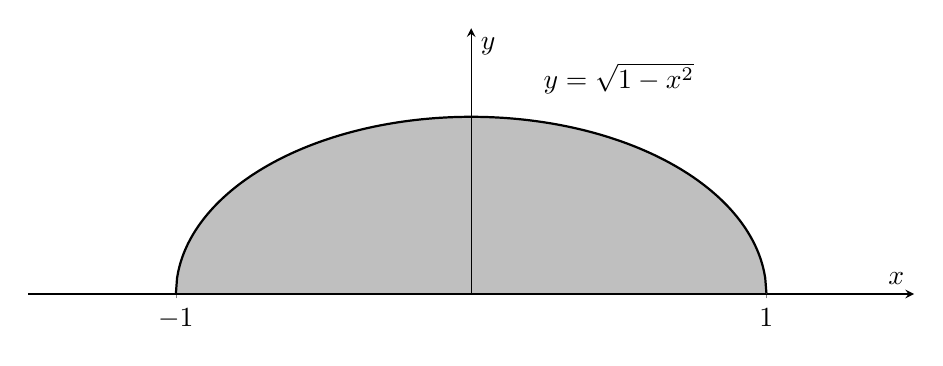
\begin{tikzpicture}[scale=0.75]
	\begin{axis}[
    		axis lines = center,
		y=3cm, % scaling y-axis
		x=5cm, % scaling x-axis
		xmax=1.5,
		xmin=-1.5,
		ymax=1.5,
		ymin=0,
   		 xlabel = \( x \),
   		 ylabel = {\( y \)},
		 xtick={-1,0,1},
    		 xticklabels={$-1$,$0$,$1$},
		 ytick={0},
		 yticklabels={$0$},
		]
		 \node (some node) at (200,100) (a) {};
		  \node (some node) at (150,200) (c) {};
	\addplot[name path=A,samples=500,domain=-1:1, color=black, style=thick]{sqrt(1-x^2)} node[above = 1 pt of a] {$y=\sqrt{1-x^2}$};
	\addplot[name path=B,thin, samples=50, smooth,domain=-1:1,black] coordinates {(-1,0)(1,0)};
	\addplot[thin, samples=50, smooth,domain=-1:1,black] coordinates {(0,0)(0,1)};
	\addplot[gray!50] fill between[of=A and B];
	\addplot [only marks] table {
};
	\end{axis}
	\end{tikzpicture}
	\end{center}
  
  By uniform distribution, $f(x,y) = 1 / \text{area}$. The area of a semi-circle with radius 1 is $\pi / 2$, so $f(x,y) = 2 / \pi$. Since
  
  \[ \rho_{xy} = \frac{E[XY] - E[X] E[Y]}{\sqrt{V[X] V[Y]}} \]
  
  First we calculate $E[XY]$:
  
  \[ E[XY] = \int^1_{-1} \int^{\sqrt{1-x^2}}_0 xy \frac{2}{\pi} \ dy \ dx = 0 \]
  
  Next, the marginal probability distributions:
  
  \begin{align*}
  g(x) &= \int^{\sqrt{1-x^2}}_0 \frac{2}{\pi} \ dy = \frac{2 \sqrt{1-x^2}}{\pi}, \quad -1 \leq x \leq 1 \\
  h(y) &= \int^{\sqrt{1-y^2}}_0 \frac{2}{\pi} \ dx + \int^0_{-\sqrt{1-y^2}} \frac{2}{\pi} \ dx = \frac{4 \sqrt{1-y^2}}{\pi}, \quad 0 \leq y \leq 1
  \end{align*}
  
  Lastly, we calculate $E[X]$ and $E[Y]$:
  
  \begin{align*}
  E[X] &= \int^1_{-1} \frac{2}{\pi} x \sqrt{1-x^2} \ dx = 0 \\
  E[Y] &= \int^1_0 \frac{4}{\pi} y \sqrt{1-y^2} \ dy \approx 0.424
  \end{align*}
  
  Therefore, $\boxed{ \rho_{xy} = 0 }$, implying $X,Y$ are uncorrelated. This does \textbf{not} mean that $X$ and $Y$ are independent, as uncorrelation does not (generally) imply independence. Note that the converse is true: independence \textbf{does} imply uncorrelation.

%Question 7.38
\item  \begin{tcolorbox}[
  colback=Cerulean!5!white,
  colframe=Cerulean!75!black]
  \textbf{Suppose that the two-dimensional random variable $\bm{(X,Y)}$ has pdf given by}
  
  \[\bm{f(x,y) =}
  \begin{dcases}
  \bm{ke^{-y},} & \bm{0 < x < y < 1} \\
  \bm{0,} & \textbf{elsewhere}
  \end{dcases} \]
  
  \textbf{Find the correlation coefficient $\bm{\rho_{xy}}$.}
  \end{tcolorbox}
  
    	\begin{center}
	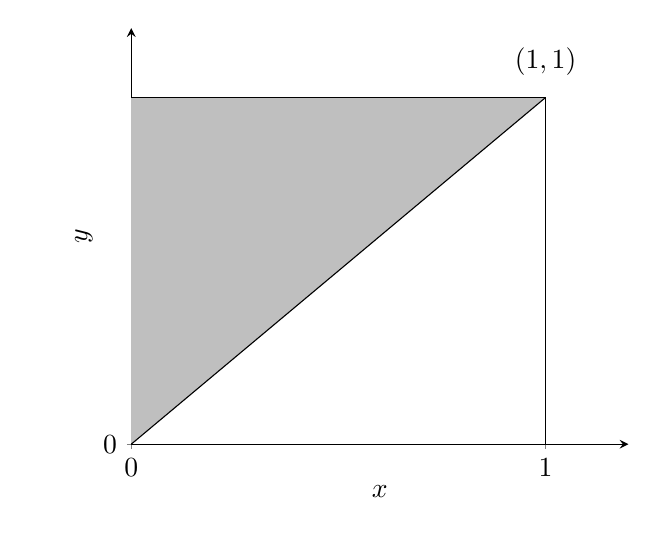
\begin{tikzpicture}[scale=0.75]
	\begin{axis}[
    		axis lines = left,
		xmax=1.2,
		xmin=0,
		ymax=1.2,
		ymin=0,
   		 xlabel = \( x \),
   		 ylabel = {\( y \)},
		 xtick={0,1},
    		 xticklabels={$0$,$1$},
		 ytick={0},
		 yticklabels={$0$,$1$},
		]
		 \node (some node) at (200,200) (a) {};
		  \node (some node) at (150,200) (c) {};
	\addplot[name path=A,samples=500,domain=-1:1, color=black, style=thin]{x} node[above = 1 pt of a] {$(1,1)$};
	\addplot[name path=B,thin, samples=50, smooth,domain=-1:1,black] coordinates {(0,1)(1,1)};
	\addplot[thin, samples=50, smooth,domain=0:1,black] coordinates {(1,0)(1,1)};
	\addplot[gray!50] fill between[of=A and B];
	\addplot [only marks] table {
};
	\end{axis}
	\end{tikzpicture}
	\end{center}

Knowing that 

\[ \rho_{xy} = \frac{E[XY] - E[X] E[Y]}{\sqrt{V[X] V[Y]}} \]

We proceed by calculating each of the constituent quantities. First, to derive $k$ in the joint pdf, we know that we must have $\int^1_0 \int^1_x ke^{-y} \ dy \ dx = 1$. Solving for $k$ yields $k = \frac{e}{e-2}$. The marginal probability distributions can now be calculated as

\begin{align*}
g(x) &= \int^1_x ke^{-y} \ dy = \frac{1}{e-2} (e^{1-x} - 1), \quad 0 \leq x \leq 1 \\
h(y) &= \int^y_0 ke^{-y} \ dx = \frac{ye^{1-y}}{e-2}, \quad 0 \leq y \leq 1
\end{align*}

Now we can calculate

\begin{align*}
E[X] &= \int^1_0 \frac{x}{e-2} (e^{1-x} - 1) \ dx \approx 0.3039 \\
E[Y] &= \int^1_0 \frac{y^2 e^{1-y}}{e-2} \ dy \approx 0.6078 \\
E[XY] &= k \int^1_0 \int^y_0 xye^{-y} \ dx \ dy \approx 0.2156 \\
V[X] &= \int^1_0 \frac{(x - E[X])^2}{e-2} (e^{1-x} - 1) \ dx \approx 0.0514 \\
V[Y] &= \int^1_0 (y - E[Y])^2 \frac{ye^{1-y}}{e - 2} \ dy \approx 0.0617
\end{align*}

Inputting the aforementioned calculations yields $\boxed{ \rho_{xy} = 0.5485 }$.

%Question 7.39
\item  \begin{tcolorbox}[
  colback=Cerulean!5!white,
  colframe=Cerulean!75!black]
  \textbf{The following example illustrates that $\bm{\rho = 0}$ does not imply independence. Suppose that $\bm{(X,Y)}$ has a joint probability distribution given by Table 7.1.}
  \end{tcolorbox}
  
  \begin{center}
\begin{tabular}{|c | c | c | c|} 
 \hline
  \diagbox{$X$\\}{\\$Y$} & $-1$ & $0$ & $1$ \\ 
 \hline\hline 
 $-1$ & $\mathcircled{\frac{1}{8}}$ & $\boxed{\frac{1}{8}}$ & $\mathcircled{\frac{1}{8}}$ \\ [1 ex] 
 \hline
 $0$ & $\boxed{\frac{1}{8}}$ & 0 & $\boxed{\frac{1}{8}}$ \\
 \hline
 $1$ & $\mathcircled{\frac{1}{8}}$ & $\boxed{\frac{1}{8}}$ & $\mathcircled{\frac{1}{8}}$ \\ 
 \hline
\end{tabular}
\end{center}

  
  	\begin{enumerate}
	%Question 7.39(a)
	\item  \begin{tcolorbox}[
	  colback=Cerulean!5!white,
	  colframe=Cerulean!75!black]
	  \textbf{Show that $\bm{E[XY] = E[X] E[Y]}$ and hence $\bm{\rho = 0}$.}
	  \end{tcolorbox}
	  
	  Calculating $E[XY], E[X], E[Y]$ gives us
	  
	  \begin{align*}
	  E[XY] &= (X = -1)(Y = -1) P(X = -1, Y = -1) + (X = -1)(Y = 1) P(X = -1, Y = 1) \\
	  &\quad + (X = 1)(Y = -1) P(X = 1, Y = -1) + (X = 1)(Y = 1) P(X = 1, Y = 1) = 0  \\
	  E[X] &= (X = -1) P(X = -1) + (X = 1) P(X = 1) = 0 \\
	  E[Y] &= (Y = -1) P(Y = -1) + (Y = 1) P(Y = 1) = 0
	  \end{align*}
	  
	  Therefore, $\boxed{E[XY] = E[X] E[Y] = 0 \implies \rho = 0}$.
	  
	  %Question 7.39(b)
	\item  \begin{tcolorbox}[
	  colback=Cerulean!5!white,
	  colframe=Cerulean!75!black]
	  \textbf{Indicate why $\bm{X}$ and $\bm{Y}$ are not independent.}
	  \end{tcolorbox}
	  
	  By definition of independence, we must have $P(X) P(Y) = P(X,Y)$. But consider $P(X = 1) P(Y = 1) = (3/8) (3/8) = 9/64$ and $P(X = 1, Y = 1) = 1/8$. Equality does not hold, and thus $X,Y$ cannot be independent.
	  
	  %Question 7.39(c)
	\item  \begin{tcolorbox}[
	  colback=Cerulean!5!white,
	  colframe=Cerulean!75!black]
	  \textbf{Show that this example may be generalized as follows. The choice of the number 1/8 is not crucial. What is important is that all the circled values are the same, all the boxed values are the same, and the center value equals zero.}
	  \end{tcolorbox}
	  
	  Let the circled values be any $a \in \mathbb{R}$ and the boxed values be any $b \in \mathbb{R}$. We can see that
	  
	  \begin{align*}
	  E[XY] &= (-1)(1) a + (-1)(1) a + (1)(-1) a + (1)(1) a = 0 \\
	  E[X] &= (X = -1) P(X = -1) + (X = 1) P(X = 1) \\
	  &= -1 (2a + b) + 1 (2a + b) = 0 \\
	  E[Y] &= (Y = -1) P(Y = -1) + (Y = 1) P(Y = 1) \\
	  &= -1 (2a + b) + 1 (2a + b) = 0
	  \end{align*}
	  
	  It follows that $E[XY] = E[X]E[Y]$ for any choice of $a, b$, and so we have $\rho = 0$. We can also see that $P(X = 1) P(Y = 1) = (2a + b)^2 = 4a^2 + 4ab + b^2$, which is not in general equal to $P(X = 1, Y = 1) = a$, and so $X,Y$ are uncorrelated but not independent.
	\end{enumerate}

%Question 7.40
\item  \begin{tcolorbox}[
  colback=Cerulean!5!white,
  colframe=Cerulean!75!black]
  \textbf{Suppose that $\bm{A}$ and $\bm{B}$ are two events associated with an experiment $\bm{\varepsilon}$. Suppose that $\bm{P(A) > 0}$ and $\bm{P(B) > 0}$. Let the random variable $\bm{X}$ and $\bm{Y}$ be defined as follows.}
  
  \begin{align*}
  \bm{X} &\bm{= 1} \textbf{ if } \bm{A} \textbf{ occurs and } \bm{0} \textbf{ otherwise} \\
  \bm{Y} &\bm{= 1} \textbf{ if } \bm{B} \textbf{ occurs and } \bm{0} \textbf{ otherwise} 
  \end{align*}
  
  \textbf{Show that $\bm{\rho_{xy} = 0}$ implies that $\bm{X}$ and $\bm{Y}$ are independent.}
  \end{tcolorbox}
  
  \begin{proof}
  By premise, we must have $E[XY] = E[X] E[Y]$. We also have $E[X] = 1 \cdot P(X = 1) = P(A)$, $E[Y] = 1 \cdot P(Y = 1) = P(B)$, and $E[XY] = (1)(1) P(X = 1, Y = 1) = P(A,B)$. Then from the premise, we have $P(A) P(B) = P(A,B)$, or $P(X = 1, Y = 1) = P(X = 1) P(Y = 1)$. From the probability table below, we can also conclude that $P(X = 1, Y = 0) = P(X = 1) P(Y = 0)$, $P(X = 0, Y = 1) = P(X = 0) P(Y = 1)$, and $P(X = 0, Y = 0) = P(X = 0) P(Y = 0)$. Therefore, $X, Y$ are independent. We have proved that \textbf{Bernoulli variables are independent if and only if they are uncorrelated} (in other words, uncorrelation \textit{also} implies independence for Bernoulli variables). 
  
\begin{center}
\begin{tabular}{|c | c | c | c |} 
 \hline
  \diagbox{$X$\\}{\\$Y$} & $0$ & $1$ & \\ 
 \hline\hline 
 $0$ & $1 - P(A) - P(B) + P(A)P(B)$ & $P(B) - P(A)P(B)$ & $= 1 - P(A)$ \\ 
 \hline
 $1$ & $P(A) - P(A)P(B)$ & $P(A)P(B)$ & = P(A) \\ 
 \hline
  & $= 1 - P(B)$ & $= P(B)$ & \\
  \hline
\end{tabular}
\end{center}
  
  \end{proof}
  
%Question 7.41
\item  \begin{tcolorbox}[
  colback=Cerulean!5!white,
  colframe=Cerulean!75!black]
  \textbf{Prove Theorem 7.14.}
  \end{tcolorbox}
  
  \begin{thm*}
  If $\rho_{xy}$ is the correlation coefficient between $X$ and $Y$, and if $V = AX + B$ and $W = CY + D$, where $A, B, C,$ and $D$ are constants, then $\rho_{vw} = (AC / |AC|) \rho_{xy}$. (We suppose that $A \neq 0$, $C \neq 0$)
  \end{thm*}
  
  \begin{proof}
  Knowing that 
  
  \[ \rho_{vw} = \frac{E[VW] - E[V] E[W]}{\sqrt{V[V] V[W]}} \]
  
  We can algebraically derive the desired result by substituting the expressions for $V$ and $W$.
  
  \begin{align*}
  \rho_{vw} &= \frac{E[ACXY + ADX + BCY + BD] - E[AX + B] E[CY + D]}{\sqrt{V[AX+B] V[CY + D]}} \\
  &= \frac{ACE[XY] + ADE[X] BCE[Y] + BD - (AE[X] + B)(CE[Y] + D)}{\sqrt{A^2 V[X] C^2 V[Y]}} \\
  &= \frac{ACE[XY] - ACE[X] E[Y]}{|AC| \sqrt{V[X] V[Y]}} \\
  &= \boxed{\frac{AC}{|AC|} \rho_{xy}}
  \end{align*}
  \end{proof}
  
%Question 7.42
\item  \begin{tcolorbox}[
  colback=Cerulean!5!white,
  colframe=Cerulean!75!black]
  \textbf{For the random variable $\bm{(X,Y)}$ defined in Problem 6.14, evaluate $\bm{E[X | y]}$, $\bm{E[Y | x]}$, and check that $\bm{E[X] = E[E[X | Y]]}$ and $\bm{E[Y] = E[E[Y | X]]}$.}
  \end{tcolorbox}
  
  Here, we verify the Law of Total Expectation. In Problem 6.14, we derived marginal pdf's $g(x) = e^{-x}, x > 0$, and $h(y) = ye^{-y}, y > 0$. Then $g(x | y) = \frac{f(x,y)}{h(y)} = \frac{1}{y}$ and $h(y | x) = \frac{f(x,y)}{g(x)} = e^{x-y}$. The expectations of $X, Y$ are 
  
  \begin{align*}
  E[X] &= \int^{+\infty}_0 x e^{-x} \ dx = \boxed{1} \\
  E[Y] &= \int^{+\infty}_0 y^2 e^{-y} \ dy = \boxed{2}
  \end{align*}
  
  Then we calculate
  
  \begin{align*}
  E[X | y] &= \int^{+\infty}_{-\infty} x g(x | y) \ dx = \int^y_0 \frac{x}{y} \ dx = \boxed{y/2} \\
  E[Y | x] &= \int^{+\infty}_{-\infty} y h(y | x) \ dy = \int^{+\infty}_x ye^{x-y} \ dy = \boxed{x + 1}
  \end{align*}
  
  Lastly, verifying that the Law of Total Expectation holds:
  
  \begin{align*}
  E[E[X | Y]] &= \int^{+\infty}_0 \frac{y}{2} (ye^{-y}) \ dy = \boxed{1} \\
  E[E[Y | X]] &= \int^{+\infty}_0 (x+1) e^{-x} \ dx = \boxed{2}
  \end{align*}
  
  Therefore, $E[X] = E[E[X | Y]]$ and $E[Y] = E[E[Y | X]]$.

%Question 7.43
\item  \begin{tcolorbox}[
  colback=Cerulean!5!white,
  colframe=Cerulean!75!black]
  \textbf{Prove Theorem 7.16.}
  \end{tcolorbox}
  
  \begin{thm*}
  Suppose that $X$ and $Y$ are independent random variables. Then
  
  \[ E[X | Y] = E[X] \quad \text{and} \quad E[Y | X] = E[Y] \]
  \end{thm*}
  
  \begin{proof}
  By independence, $f(x,y) = g(x) h(y)$. Then we can derive
  
  \begin{align*}
  E[X | Y] &= \int^{+\infty}_{-\infty} x g(x | y) \ dx = \int^{+\infty}_{-\infty} x \frac{f(x,y)}{h(y)} \ dx = \int^{+\infty}_{-\infty} x g(x) \ dx = E[X] \\
  E[Y | X] &= \int^{+\infty}_{-\infty} y h(y | x) \ dy = \int^{+\infty}_{-\infty} y \frac{f(x,y)}{g(x)} \ dy = \int^{+\infty}_{-\infty} y h(y) \ dy = E[Y]
  \end{align*}
  \end{proof}
  
%Question 7.44
\item  \begin{tcolorbox}[
  colback=Cerulean!5!white,
  colframe=Cerulean!75!black]
  \textbf{Prove Theorem 7.17. [\textit{Hint:} For the continuous case, multiply the equation $\bm{E[Y | x] = Ax + B}$ by $\bm{g(x)}$, the pdf of $\bm{X}$, and integrate from $\bm{-\infty}$ to $\bm{\infty}$. Do the same thing, using $\bm{xg(x)}$ and then solve the resulting two equations for $\bm{A}$ and for $\bm{B}$.]}
  \end{tcolorbox}
  
  \begin{thm*}
  Let $(X,Y)$ be a two-dimensional random variable and suppose that
  
  \[ E[X] = \mu_x \quad E[Y] = \mu_y \quad V[X] = \sigma^2_x \quad V[Y] = \sigma^2_y \]
  
  Let $\rho$ be the correlation coefficient between $X$ and $Y$. If the regression of $Y$ on $X$ is linear, we have
  
  \[ E[Y | x] = \mu_y + \rho \frac{\sigma_y}{\sigma_x} (x - \mu_x) \]
  
  If the regression of $X$ on $Y$ is linear, we have
  
  \[ E[X | y] = \mu_x + \rho \frac{\sigma_x}{\sigma_y} (y - \mu_y) \]
    
  \end{thm*}
  
  \begin{proof}
  \textbf{Continuous case.} Let $E[Y | x] = Ax + B$. We must attempt to show that $A = \rho \frac{\sigma_y}{\sigma_x}$ and $B = \mu_y -\mu_x \rho \frac{\sigma_y}{\sigma_x}$. Observe that
  
  \begin{align*}
  E[Y] = \mu_y &= \int^{+\infty}_{-\infty} E[Y | x] g(x) \ dx \\
  &= \int^{+\infty}_{-\infty} (Ax + B) g(x) \ dx \\
  &= \int^{+\infty}_{-\infty} Ax g(x) \ dx + \int^{+\infty}_{-\infty} B g(x) \ dx \\
  &= A \mu_x + B
  \end{align*}
  
  Now, consider the integral
  
  \begin{align*}
  \int^{+\infty}_{-\infty} E[Y | x] x g(x) \ dx &= \int^{+\infty}_{-\infty} (Ax + B) x g(x) \ dx \\
  &= \int^{+\infty}_{-\infty} Ax^2 g(x) \ dx + \int^{+\infty}_{-\infty} B x g(x) \ dx \\
  &= A E[X^2] + B \mu_x
  \end{align*}
  
  which is also equal to
  
  \begin{align*}
  \int^{+\infty}_{-\infty} E[Y | x] x g(x) \ dx &= \int^{+\infty}_{-\infty} \Bigg( \int^{+\infty}_{-\infty} y h(y | x) \ dy \Bigg) x g(x) \ dx \\
  &= \int^{+\infty}_{-\infty} \Bigg( \int^{+\infty}_{-\infty} y \frac{f(x,y)}{g(x)} \ dy \Bigg) x g(x) \ dx \\
  &= \int^{+\infty}_{-\infty} \int^{+\infty}_{-\infty} xy f(x,y) \ dy \ dx \\
  &= E[XY]
  \end{align*}
  
  Thus we are left with the system of equations
  
  \begin{align*}
  A \mu_x + B &= \mu_y \\
  A E[X^2] + B \mu_x &= E[XY]
  \end{align*}
  
  Solving for $A$ and $B$ yields
  
  \[ A = \frac{Cov(X,Y)}{V[X]} = \boxed{\rho \frac{\sigma_y}{\sigma_x}} \quad B = \mu_y - \frac{Cov(X,Y)}{V[X]} \mu_x = \boxed{\mu_y - \mu_x \rho \frac{\sigma_y}{\sigma_x}} \]
  
  \textbf{Discrete case.} The strategy is simply to replicate what we did in the continuous case, but using summations. First consider
  
  \begin{align*}
  E[Y | x_j] &= \sum_i y_i P(y_i | x_j) \\
  &= \sum_i y_i \frac{P(y_i, x_j)}{P(x_j)}
  \end{align*}
  
  Now suppose that $E[Y | x_j] = Ax_j + B$. Taking the expectation of each side (i.e. summing through each of the discrete values of the $x_j's$) gives us
  
  \begin{align*}
  \sum_j \sum_i y_i P(y_i, x_j) &= \sum_j (A x_j P(x_j) + B P(x_j)) \\
  \implies \mu_y &= A \mu_x + B
  \end{align*}
  
  Analogous to the continuous case, we also see that
  
  \begin{align*}
  \sum_j \sum_i y_i P(y_i, x_j) x_j &= \sum_j (A x^2_j P(x_j) + B x_j P(x_j)) \\
  \implies E[XY] &= A E[X^2] + B \mu_x
  \end{align*}
  
  Leaving us with the same system equations as in the continuous case:
  
  \begin{align*}
  A \mu_x + B &= \mu_y \\
  A E[X^2] + B \mu_x &= E[XY]
  \end{align*}
  
  Solve for $A$ and $B$ as before and this finishes the proof for the discrete case.
  
  \end{proof}
  
%Question 7.45
\item  \begin{tcolorbox}[
  colback=Cerulean!5!white,
  colframe=Cerulean!75!black]
  \textbf{Prove Theorem 7.18.}
  \end{tcolorbox}
  
  \begin{thm*}
  If $y = ax + b$ is the least-squares approximation to $E[Y | x]$ and if $E[Y | x]$ is in fact a linear function of $x$, that is
  
  \[ E[Y | x] = a'x + b' \]
  
  then $a = a'$ and $b = b'$. An analogous statement holds for the regression of $X$ on $Y$.
  \end{thm*}
  
  By premise, $a,b$ are such that $E[(E[Y | X] - (aX + b))^2] = E[((a'X + b') - (aX + b))^2]$ is minimized. Expanding, the expression, we find
  
  \begin{align*}
  E[((a'X + b') - (aX + b))^2] &= E[((a' - a)X + (b' - b))^2] \\
  &= E[(a'-a)^2 X^2 + 2(a' - a)(b' - b) X = (b' - b)^2] \\
  &= (a' - a)^2 E[X^2] + 2(a' - a) (b' - b) E[X] + (b' - b)^2
  \end{align*}
  
  Observe that $(a' - a)^2 \geq 0$, as does $E[X^2] \geq 0$ (an average of exclusively zero or positive values is necessarily zero or positive) and $(b' - b)^2 \geq 0$. Since we wish to minimize the above expression, it follows that the only way to do so is for $a' - a = b' - b = 0$. Then $E[(E[Y | X] - (aX + b))^2] = 0$, which is indeed the lowest value it can take given that the argument of the expectation is a square term, and $a' = a, b' = b$.

%Question 7.46
\item  \begin{tcolorbox}[
  colback=Cerulean!5!white,
  colframe=Cerulean!75!black]
  \textbf{If $\bm{X}$, $\bm{Y}$, and $\bm{Z}$ are uncorrelated random variables with standard deviations 5, 12, and 9, respectively and if $\bm{U = X + Y}$ and $\bm{V = Y + Z}$, evaluate the correlation coefficient between $\bm{U}$ and $\bm{V}$.}
  \end{tcolorbox}
  
  We must calculate the constituent quantities that comprise
  
  \[ \rho_{uv} = \frac{E[UV] - E[U] E[V]}{\sqrt{V[V] V[U]}} \]
  
  By premise, $\sigma_x = 5, \sigma_y = 12, \sigma_z = 9$, and $\rho_{xy} = \rho_{yz} = \rho_{xz} = 0$. This also means
  
  \begin{align*}
  \sigma^2_x &= V[X] = E[X^2] - E[X]^2 = 25 \\
  \sigma^2_y &= V[Y] = E[Y^2] - E[Y]^2 = 144 \\
  \sigma^2_z &= V[Z] = E[Z^2] - E[Z]^2 = 81 \\
  E[XY] &= E[X] E[Y] \\
  E[YZ] &= E[Y] E[Z] \\
  E[XZ] &= E[X] E[Z]
  \end{align*}
  
  Now, the expectations for the $U, V$ quantities are given by
  
  \begin{align*}
  E[U] &= E[X] + E[Y] \\
  E[V] &= E[Y] + E[Z] \\
  E[U] E[V] &= E[X] E[Y] + E[X] E[Z] + E[Y]^2 + E[Y] E[Z] \\
  E[UV] &= E[XY] + E[XZ] + E[Y^2] + E[YZ] \\
  E[U^2] &= E[X^2] + 2E[XY] + E[Y^2] \\
  E[V^2] &= E[Y^2] + 2E[YZ] + E[Z^2]
  \end{align*}
  
  Lastly, we can calculate $\rho_{uv}$. First the numerator:
  
  \begin{align*}
  E[UV] - E[U] E[V] &= (E[XY] - E[X]E[Y]) + (E[XZ] - E[X] E[Z]) + (E[YZ] - E[Y] E[Z]) + (E[Y^2] - E[Y]^2) \\
  &= E[Y^2] - E[Y]^2 = 144
  \end{align*}
  
  And now $V[V]$ and $V[U]$:
  
  \begin{align*}
  V[U] &= E[U^2] - E[U]^2 \\
  &= E[X^2] + 2E[XY] + E[Y^2] - (E[X]^2 + 2E[X] E[Y] + E[Y]^2) \\
  &= (E[X^2] - E[X]^2) + 2(E[XY] - E[X] E[Y]) + (E[Y^2] - E[Y]^2)  \\
  &= 25 + 144 = 169 \\
  V[V] &= E[V^2] - E[V]^2 \\
  &= E[Y^2] + 2E[YZ] + E[Z^2] - (E[Y]^2 + 2E[Y] E[Z] + E[Z]^2) \\
  &= (E[Y^2] - E[Y]^2) + 2(E[YZ] - E[Y] E[Z]) + (E[Z^2] - E[Z]^2) \\
  &= 144 + 81 = 225
  \end{align*}
  
  Inputting the aforementioned values gets us
  
  \[ \rho_{uv} = \frac{E[UV] - E[U] E[V]}{\sqrt{V[V] V[U]}} = \frac{144}{\sqrt{169 \cdot 225}} = \boxed{ \frac{48}{65} } \]

%Question 7.47
\item  \begin{tcolorbox}[
  colback=Cerulean!5!white,
  colframe=Cerulean!75!black]
  \textbf{Suppose that both of the regression curves of the mean are in fact linear. Specifically, assume that $\bm{E[Y | x] = -\frac{3}{2} x - 2}$ and $\bm{E[X | y] = -\frac{3}{5} y - 3}$.}
  \end{tcolorbox}
  
	\begin{enumerate}
	%Question 7.47(a)
	\item  \begin{tcolorbox}[
	  colback=Cerulean!5!white,
	  colframe=Cerulean!75!black]
	  \textbf{Determine the correlation coefficient $\bm{\rho}$.}
	  \end{tcolorbox}
	  
	  By Meyer Theorem 7.17, if the regressions of $Y$ on $X$ and vice-versa are linear, then we can write
	  
	  \begin{align*}
	  E[Y | x] &= \mu_y + \rho \frac{\sigma_y}{\sigma_x} (x - \mu_x) \\
	  &= \mu_y - \rho \frac{\sigma_y}{\sigma_x} \mu_x + \rho \frac{\sigma_y}{\sigma_x} x \\
	  E[X | y] &= \mu_x + \rho \frac{\sigma_x}{\sigma_y} (y - \mu_y) \\
	  &= \mu_x - \rho \frac{\sigma_x}{\sigma_y} \mu_y + \rho \frac{\sigma_x}{\sigma_y} y
	  \end{align*}
	  
	  It then follows that $\rho \frac{\sigma_y}{\sigma_x} = -3/2$ and $\rho \frac{\sigma_x}{\sigma_y} = -3/5$. Multiplying the expressions yields $\rho^2 = 9/10$, allowing us to conclude that $\boxed{ \rho = -3 / \sqrt{10} }$. The correlation must be negative, for $\sigma_x, \sigma_y$ are necessarily positive.
	  
	  %Question 7.47(b)
	\item  \begin{tcolorbox}[
	  colback=Cerulean!5!white,
	  colframe=Cerulean!75!black]
	  \textbf{Determine $\bm{E[X]}$ and $\bm{E[Y]}$.}
	  \end{tcolorbox}
	  
	  By the Law of Total Expectation, $E[E[X | Y]] = E[X]$ and $E[E[Y | X]] = E[Y]$. We solve the system of equations
	  
	  \begin{align*}
	  E[E[Y | X]] &= -\frac{3}{2} E[X] - 2 = E[Y] \\
	  E[E[X | Y]] &= -\frac{3}{5} E[Y] - 3 = E[X] \\
	  \end{align*}
	  \begin{align*}
	  \implies &-\frac{3}{2} \Big( -\frac{3}{5} E[Y] - 3 \Big) - 2 = E[Y] \\
	  \implies &\boxed{E[Y] = 25, E[X] = -18}
	  \end{align*}
	  
	  
	  
	\end{enumerate}

\newpage
%Question 7.48
\item  \begin{tcolorbox}[
  colback=Cerulean!5!white,
  colframe=Cerulean!75!black]
\textbf{Consider weather forecasting with two alternatives: ``rain" or ``no rain" in the next 24 hours. Suppose that $\bm{p = }$ Prob(rain in the next 24 hours) $\bm{> 1/2}$. The forecaster scores 1 point if he is correct and 0 points if not. In making $\bm{n}$ forecasts, a forecaster with no ability whatsoever chooses at random $\bm{r}$ days $\bm{(0 \leq r \leq n)}$ to say ``rain" and the remaining $\bm{n-r}$ days to say ``no rain." His total point score is $\bm{S_n}$. Compute $\bm{E[S_n]}$ and $\bm{Var[S_n]}$ and find that value of $\bm{r}$ for which $\bm{E[S_n]}$ is largest. [Hint: $\bm{X_1 = 1}$ or 0 depending on whether the $\bm{i}$-th forecast is correct or not. Then $\bm{S_n = \sum^n_{i=1} X_i}$. Note that the $\bm{X_i}$'s are \textit{not} independent.] }
\end{tcolorbox}

This is a classic Markov chain problem, but Meyer is asking us to use only the elementary notions we have learned thus far without the advanced tools of transition matrices and state spaces. Challenge accepted.

Our first point of order is to recognize that we are attempting to model a \textbf{path-dependent process}. We have determined a priori that we will predict that it will rain $r$ times. In our prediction for the first day, we randomly prognosticate whether it rains or not, in a manner as if we had a hat full of $r$ slips of paper that said ``rain," and $n-r$ slips that said ``no rain." Whichever we draw is our prediction for that day. 

Should we say it rains on the first day, however, then in our prediction for the second day, we will only have $r-1$ slips that say ``rain" to pick from, and still $n-r$ slips of ``no rain." 

In a counterfactual scenario, we drew ``no rain" in predicting the first day's weather, and now we are left with $r$ ``rains" and $n-r-1$ ``no rains." And this process continues until we have exhausted all of the $n$ slips of paper. 

Clearly, where we end up on each day of predictions is contingent on \textit{how we predicted on all previous days.} Hence the path-dependency.

\end{enumerate}

\end{document}